% Template adapted from https://github.com/jgm/pandoc-templates/blob/master/default.latex
% To be used with XeLaTex in memoiR
%%%%%%%%%%%%%%%%%%%%%%%%%%%%%%%%%%%%%%%%%%%%%%%%%%%%%%%%%%%%%%%%%%%%%%%%%%%%%%%%%%%%%%%%%

% Options for packages loaded elsewhere
\PassOptionsToPackage{unicode=true}{hyperref}
\PassOptionsToPackage{hyphens}{url}
\PassOptionsToPackage{dvipsnames,svgnames*,x11names*}{xcolor}
% Right to left support


\documentclass[
  11pt,
  italian,
  a4paper,
  extrafontsizes,onecolumn,openright
  ]{memoir}

% Double (or whatever) spacing

% Math
\usepackage{amssymb, amsmath}
% mathspec: arbitrary math fonts
\usepackage{unicode-math}
\defaultfontfeatures{Scale=MatchLowercase}
\defaultfontfeatures[\rmfamily]{Ligatures=TeX,Scale=1}

% Fonts
\usepackage{lmodern}
\usepackage{fontspec}

% Main font
% Specific sanserif font
% Specific monotype font
\setmonofont[Scale=0.85]{Inconsolata}
% Specific math font
% Chinese, Japanese, Corean fonts

% Use upquote for straight quotes in verbatim environments
\usepackage{upquote}
% Use microtype
\usepackage[]{microtype}
\UseMicrotypeSet[protrusion]{basicmath} % disable protrusion for tt fonts

% Verbatim in note

% Color links
\usepackage{xcolor}

% Strikeout

% Necessary for code chunks
\usepackage{color}
\usepackage{fancyvrb}
\newcommand{\VerbBar}{|}
\newcommand{\VERB}{\Verb[commandchars=\\\{\}]}
\DefineVerbatimEnvironment{Highlighting}{Verbatim}{commandchars=\\\{\}}
% Add ',fontsize=\small' for more characters per line
\usepackage{framed}
\definecolor{shadecolor}{RGB}{248,248,248}
\newenvironment{Shaded}{\begin{snugshade}}{\end{snugshade}}
\newcommand{\AlertTok}[1]{\textcolor[rgb]{0.94,0.16,0.16}{#1}}
\newcommand{\AnnotationTok}[1]{\textcolor[rgb]{0.56,0.35,0.01}{\textbf{\textit{#1}}}}
\newcommand{\AttributeTok}[1]{\textcolor[rgb]{0.77,0.63,0.00}{#1}}
\newcommand{\BaseNTok}[1]{\textcolor[rgb]{0.00,0.00,0.81}{#1}}
\newcommand{\BuiltInTok}[1]{#1}
\newcommand{\CharTok}[1]{\textcolor[rgb]{0.31,0.60,0.02}{#1}}
\newcommand{\CommentTok}[1]{\textcolor[rgb]{0.56,0.35,0.01}{\textit{#1}}}
\newcommand{\CommentVarTok}[1]{\textcolor[rgb]{0.56,0.35,0.01}{\textbf{\textit{#1}}}}
\newcommand{\ConstantTok}[1]{\textcolor[rgb]{0.00,0.00,0.00}{#1}}
\newcommand{\ControlFlowTok}[1]{\textcolor[rgb]{0.13,0.29,0.53}{\textbf{#1}}}
\newcommand{\DataTypeTok}[1]{\textcolor[rgb]{0.13,0.29,0.53}{#1}}
\newcommand{\DecValTok}[1]{\textcolor[rgb]{0.00,0.00,0.81}{#1}}
\newcommand{\DocumentationTok}[1]{\textcolor[rgb]{0.56,0.35,0.01}{\textbf{\textit{#1}}}}
\newcommand{\ErrorTok}[1]{\textcolor[rgb]{0.64,0.00,0.00}{\textbf{#1}}}
\newcommand{\ExtensionTok}[1]{#1}
\newcommand{\FloatTok}[1]{\textcolor[rgb]{0.00,0.00,0.81}{#1}}
\newcommand{\FunctionTok}[1]{\textcolor[rgb]{0.00,0.00,0.00}{#1}}
\newcommand{\ImportTok}[1]{#1}
\newcommand{\InformationTok}[1]{\textcolor[rgb]{0.56,0.35,0.01}{\textbf{\textit{#1}}}}
\newcommand{\KeywordTok}[1]{\textcolor[rgb]{0.13,0.29,0.53}{\textbf{#1}}}
\newcommand{\NormalTok}[1]{#1}
\newcommand{\OperatorTok}[1]{\textcolor[rgb]{0.81,0.36,0.00}{\textbf{#1}}}
\newcommand{\OtherTok}[1]{\textcolor[rgb]{0.56,0.35,0.01}{#1}}
\newcommand{\PreprocessorTok}[1]{\textcolor[rgb]{0.56,0.35,0.01}{\textit{#1}}}
\newcommand{\RegionMarkerTok}[1]{#1}
\newcommand{\SpecialCharTok}[1]{\textcolor[rgb]{0.00,0.00,0.00}{#1}}
\newcommand{\SpecialStringTok}[1]{\textcolor[rgb]{0.31,0.60,0.02}{#1}}
\newcommand{\StringTok}[1]{\textcolor[rgb]{0.31,0.60,0.02}{#1}}
\newcommand{\VariableTok}[1]{\textcolor[rgb]{0.00,0.00,0.00}{#1}}
\newcommand{\VerbatimStringTok}[1]{\textcolor[rgb]{0.31,0.60,0.02}{#1}}
\newcommand{\WarningTok}[1]{\textcolor[rgb]{0.56,0.35,0.01}{\textbf{\textit{#1}}}}

% Listings package

% Tables
\usepackage{longtable,booktabs,tabu}
% Fix footnotes in tables (requires footnote package)
\IfFileExists{footnote.sty}{\usepackage{footnote}\makesavenoteenv{longtable}}{}

% Graphics
\usepackage{graphicx,grffile}
\graphicspath{{images/}}
\makeatletter
\def\maxwidth{\ifdim\Gin@nat@width>\linewidth\linewidth\else\Gin@nat@width\fi}
\def\maxheight{\ifdim\Gin@nat@height>\textheight\textheight\else\Gin@nat@height\fi}
\makeatother
% Scale images if necessary, so that they will not overflow the page
% margins by default, and it is still possible to overwrite the defaults
% using explicit options in \includegraphics[width, height, ...]{}
\setkeys{Gin}{width=\maxwidth,height=\maxheight,keepaspectratio}

% Prevent overfull lines
\setlength{\emergencystretch}{3em}  
\providecommand{\tightlist}{%
  \setlength{\itemsep}{0pt}\setlength{\parskip}{0pt}}

% Number sections for memoir (secnumdepth counter is ignored)
\setsecnumdepth{section}

% Set default figure placement to htbp
\makeatletter
\def\fps@figure{htbp}
\makeatother

% Spacing in lists
\usepackage{enumitem}

% Polyglossia
\usepackage{polyglossia}
\setmainlanguage{it}
\setotherlanguage{en-US}

% BibLaTeX
\usepackage[backend=biber,style=authoryear-ibid,isbn=false,backref=true,giveninits=true,uniquename=init,maxcitenames=2,maxbibnames=150,sorting=nyt,sortcites=false]{biblatex}
\addbibresource{refs.bib}

% cslreferences environment required by pandoc > 2.7



%%%%%%%%%%%%%%%%%%%%%%%%%%%%%%%%%%%%%%%%%%%%%%%%%%%%%%%%%%
% memoiR format

% Chapter Summary environment 
\usepackage[tikz]{bclogo}
\newenvironment{Summary}
  {\begin{bclogo}[logo=\bctrombone, noborder=true, couleur=lightgray!50]{In breve}\parindent0pt}
  {\end{bclogo}}
% Syntax:
%
%```{block, type='Summary'}
% Deliver message here.
% ```

% scriptsize code 
\let\oldverbatim\verbatim
\def\verbatim{\oldverbatim\scriptsize}
% Applies to code blocks and R code results
% code chunk options size='scriptsize' applies only to R code and results
% if the code chunk sets a different size, \def\verbatim{...} is prioritary for code results 


% Layout
%%%%%%%%%%%%%%%%%%%%%%%%%%%%%%%%%%%%%%%%%%%%%%%%%%%%%%%%%%

% Based on memoir, style companion
\newcommand{\MemoirChapStyle}{daleif1}
\newcommand{\MemoirPageStyle}{Ruled}

% Space between paragraphs
\usepackage{parskip}
  \abnormalparskip{3pt}

% Adjust margin paragraphs vertical position
\usepackage{marginfix}


% Margins
%%%%%%%%%%%%%%%%%%%%%%%%%%%%%%%%%%%%%%%

% allow use of '-',+','/' ans '*' to make simple length computation
\usepackage{calc}

% Full-width figures utilities
\newlength\widthw % full width
\newlength{\rf}
\newcommand*{\definesHSpace}{
  \strictpagecheck % slower but efficient detection of odd/even pages
  \checkoddpage
  \ifoddpage
  \setlength{\rf}{0mm}
  \else
  \setlength{\rf}{\marginparsep+\marginparwidth}
  \fi
}

\makeatletter
% 1" margins for the front matter.
\newcommand*{\SmallMargins}{
  \setlrmarginsandblock{1.5in}{1.5in}{*}
  \setmarginnotes{0.1in}{0.1in}{0.1in}
 \setulmarginsandblock{1.5in}{1in}{*}
  \checkandfixthelayout
  \ch@ngetext
  \clearpage
  \setlength{\widthw}{\textwidth+\marginparsep+\marginparwidth}
  \footnotesatfoot
  \chapterstyle{\MemoirChapStyle}  % Chapter and page styles must be recalled
  \pagestyle{\MemoirPageStyle}
}

% 3" outer margin for the main matter
\newcommand{\LargeMargins}{\SmallMargins}
\makeatother

% Figure captions and footnotes in outer margins


% Main title page with filigrane
%%%%%%%%%%%%%%%%%%%%%%%%%%%%%%%%%%%%%%%%%%%%%%%%%%%%%%%%%%

% Text blocks
\usepackage[absolute,overlay]{textpos}
  \setlength{\TPHorizModule}{1mm}
  \setlength{\TPVertModule}{1mm}

\newcommand{\MainTitlePage}[2]{
  \SmallMargins % Margins
  \pagestyle{empty} % No header/footer
  \textblockorigin{\stockwidth-\paperwidth-\trimedge}{\trimtop} % recto
  \begin{textblock*}{2mm}(\spinemargin/2,\uppermargin/2)
    \rule{1pt}{\paperheight-\uppermargin}
  \end{textblock*}
  \begin{textblock*}{\paperwidth*2/3}(\paperwidth/5, \paperheight/5)
    \flushright
    \begin{Spacing}{3}
      {\fontfamily{qtm}\selectfont\fontsize{45}{45}\selectfont\textsc{\thetitle}}
    \end{Spacing}
  \end{textblock*}
    \begin{textblock*}{\paperwidth*2/3}(\paperwidth/5, \paperheight/2)
    \flushright
    {\fontfamily{qtm}\huge\theauthor}
  \end{textblock*}
    \begin{textblock*}{\paperwidth*2/3}[0, 1](\spinemargin, \uppermargin+\textheight)
    \normalfont\thedate
  \end{textblock*}
  ~\\ % Print a character or the page will not exist
  \newpage
  \textblockorigin{\trimedge}{\trimtop} % verso
  \begin{textblock*}{\textwidth}(\paperwidth-\spinemargin-\textwidth, \uppermargin)
    #1
  \end{textblock*}
  \begin{textblock*}{\textwidth}[0,1](\paperwidth-\spinemargin-\textwidth, \uppermargin+\textheight+\footskip)
    \centering
    
\includegraphics[width=\paperwidth/4]{logo}\\ \bigskip
    #2
  \end{textblock*}
  ~\\ % Print a character or the page will not exist
  \newpage
}

% Clear page and open an even one (\clearpage opens an odd one)
\newcommand{\evenpage}{
  \clearpage
  \strictpagecheck % slower but efficient detection of odd/even pages
  \checkoddpage
  \ifoddpage
    \thispagestyle{empty}
    ~\\ % Print a character or the page will not exist
    \newpage
  \else
    % do nothing
  \fi
}


%% PDF title page to insert
%%%%%%%%%%%%%%%%%%%%%%%%%%%%%%%%%%%%%%%%%%%%%%%%%%%%%%%%%%



%% Bibliography
%%%%%%%%%%%%%%%%%%%%%%%%%%%%%%%%%%%%%%%%%%%%%%%%%%%%%%%%%%

\usepackage[strict,autostyle]{csquotes}
% Repeated citation as author-year-title instead of author-title (modification of footcite:note in verbose-inote.cbx)

%% Table of Contents
%%%%%%%%%%%%%%%%%%%%%%%%%%%%%%%%%%%%%%%%%%%%%%%%%%%%%%%%%%

% fix the typesetting of the part number
\renewcommand\partnumberlinebox[2]{#2\ ---\ }


% Fonts
%%%%%%%%%%%%%%%%%%%%%%%%%%%%%%%%%%%%%%%%%%%%%%%%%%%%%%%%%%


% Hyperref comes last
%%%%%%%%%%%%%%%%%%%%%%%%%%%%%%%%%%%%%%%%%%%%%%%%%%%%%%%%%%

\usepackage{hyperref}
\hypersetup{
  pdftitle={Psicometria},
  pdfauthor={Corrado Caudek},
  colorlinks=true,
  linkcolor=Maroon,
  citecolor=Blue,
  urlcolor=Blue,
  breaklinks=true}

% Don't use monospace font for urls
\urlstyle{same}


% Title, author, date from YAML to LaTeX
%%%%%%%%%%%%%%%%%%%%%%%%%%%%%%%%%%%%%%%%%%%%%%%%%%%%%%%%%%

\title{Psicometria}

\author{Corrado Caudek}

\date{2021-10-16}


% Include headers (preamble.tex) here
%%%%%%%%%%%%%%%%%%%%%%%%%%%%%%%%%%%%%%%%%%%%%%%%%%%%%%%%%%
% Add LaTeX code into the preamble of the document here
\hyphenation{bio-di-ver-si-ty sap-lings}


%%%%%%%%%%%%%%%%%%%%%%%%%%%%%%%%%%%%%%%%%%%%%%%%%%%%%%%%%%%%%%%%%%%%%%%%%
% memoiR dalef3 chapter style 
% https://ctan.crest.fr/tex-archive/info/latex-samples/MemoirChapStyles/MemoirChapStyles.pdf
\usepackage{soul}
\definecolor{nicered}{rgb}{.647,.129,.149}
\makeatletter
\newlength\dlf@normtxtw
\setlength\dlf@normtxtw{\textwidth}
\def\myhelvetfont{\def\sfdefault{mdput}}
\newsavebox{\feline@chapter}
\newcommand\feline@chapter@marker[1][4cm]{%
  \sbox\feline@chapter{%
    \resizebox{!}{#1}{\fboxsep=1pt%
	  \colorbox{nicered}{\color{white}\bfseries\sffamily\thechapter}%
	}}%
  \rotatebox{90}{%
    \resizebox{%
	  \heightof{\usebox{\feline@chapter}}+\depthof{\usebox{\feline@chapter}}}%
	{!}{\scshape\so\@chapapp}}\quad%
  \raisebox{\depthof{\usebox{\feline@chapter}}}{\usebox{\feline@chapter}}%
 }
\newcommand\feline@chm[1][4cm]{%
  \sbox\feline@chapter{\feline@chapter@marker[#1]}%
  \makebox[0pt][l]{% aka \rlap
    \makebox[1cm][r]{\usebox\feline@chapter}%
  }}
\makechapterstyle{daleif1}{
  \renewcommand\chapnamefont{\normalfont\Large\scshape\raggedleft\so}
  \renewcommand\chaptitlefont{\normalfont\huge\bfseries\scshape\color{nicered}}
  \renewcommand\chapternamenum{}
  \renewcommand\printchaptername{}
  \renewcommand\printchapternum{\null\hfill\feline@chm[2.5cm]\par}
  \renewcommand\afterchapternum{\par\vskip\midchapskip}
  \renewcommand\printchaptertitle[1]{\chaptitlefont\raggedleft ##1\par}
}
\makeatother

\DeclareMathOperator{\Var}{Var} % Define variance operator
\DeclareMathOperator{\SD}{SD} % Define sd operator
\DeclareMathOperator{\Cov}{Cov} % Define covariance operator
\DeclareMathOperator{\Corr}{Corr} % Define correlation operator
\DeclareMathOperator{\Me}{Me} % Define mediane operator
\DeclareMathOperator{\Mo}{Mo} % Define mode operator
\DeclareMathOperator{\Bin}{Bin} % Define binomial operator
\DeclareMathOperator{\Bernoulli}{Bernoulli} % Define Bernoulli operator
\DeclareMathOperator{\Poi}{Poi} % Define Poisson operator
\DeclareMathOperator{\Uniform}{Uniform} % Define Uniform operator
\DeclareMathOperator{\Cauchy}{Cauchy} % Define Cauchy operator
\DeclareMathOperator{\elpd}{elpd} % Define elpd operator
\DeclareMathOperator{\lppd}{lppd} % Define lppd operator
\DeclareMathOperator{\LOO}{LOO} % Define LOO operator
\DeclareMathOperator{\B}{\mathscr{B}} % Define Bernoulli operator
\newcommand{\R}{\textsf{R}} % Define R programming language symbol
\newcommand{\E}{\mathbb{E}} % Define expected value operator
\newcommand{\Real}{\mathbb{R}} % Define real number operator
\newcommand{\Prob}{\mathscr{P}}
\DeclareMathOperator*{\argmin}{arg\,min} % thin space, limits on side in displays
\DeclareMathOperator*{\argmax}{arg\,max} % thin space, limits on side in displays

\raggedbottom % allow variable (ragged) site heights
\frenchspacing

\usepackage[
  labelfont=bf, 
  font={small, it} 
]{caption} 
\usepackage{upquote} % print correct quotes in verbatim-environments
\usepackage{empheq} 
\usepackage{xfrac}





\usepackage{booktabs}
\usepackage{longtable}
\usepackage{array}
\usepackage{multirow}
\usepackage{wrapfig}
\usepackage{float}
\usepackage{colortbl}
\usepackage{pdflscape}
\usepackage{tabu}
\usepackage{threeparttable}
\usepackage{threeparttablex}
\usepackage[normalem]{ulem}
\usepackage{makecell}
\usepackage{xcolor}


% End of preamble
%%%%%%%%%%%%%%%%%%%%%%%%%%%%%%%%%%%%%%%%%%%%%%%%%%%%%%%%%%


\begin{document}
\frontmatter

% Title page
%%%%%%%%%%%%%%%%%%%%%%%%%%%%%%%%%%%%%%%%%%%%%%%%%%%%%%%%%%


\MainTitlePage{Questo documento è stato realizzato con:

\begin{itemize}
  \item \LaTeX\; e la classe memoir (\url{http://www.ctan.org/pkg/memoir});
  \item $\R$ (\url{http://www.r-project.org/}) e RStudio (\url{http://www.rstudio.com/});
  \item bookdown (\url{http://bookdown.org/}) e memoiR (\url{https://ericmarcon.github.io/memoiR/}).
\end{itemize}}{Nel blog della mia pagina personale sono forniti alcuni approfondimenti degli argomenti qui trattati.

\url{https://ccaudek.github.io/caudeklab/}}


% Before Body
%%%%%%%%%%%%%%%%%%%%%%%%%%%%%%%%%%%%%%%%%%%%%%%%%%%%%%%%%%





% Contents
%%%%%%%%%%%%%%%%%%%%%%%%%%%%%%%%%%%%%%%%%%%%%%%%%%%%%%%%%%

\LargeMargins
{
\hypersetup{linkcolor=}
\setcounter{tocdepth}{2}
\tableofcontents
}


% Body
%%%%%%%%%%%%%%%%%%%%%%%%%%%%%%%%%%%%%%%%%%%%%%%%%%%%%%%%%%

\LargeMargins
\hypertarget{prefazione}{%
\chapter{Prefazione}\label{prefazione}}

\textbf{Data Science per psicologi} contiene il materiale delle lezioni dell'insegnamento di \emph{Psicometria B000286} (A.A. 2021/2022) rivolto agli studenti del primo anno del Corso di Laurea in Scienze e Tecniche Psicologiche dell'Università degli Studi di Firenze.

L'insegnamento di Psicometria si propone di fornire agli studenti un'introduzione all'analisi dei dati in psicologia.
Le conoscenze/competenze che verranno sviluppate in questo insegnamento sono quelle della \emph{Data science}, ovvero le conoscenze/competenze che si pongono all'intersezione tra statistica (ovvero, richiedono la capacità di comprendere teoremi statistici) e informatica (ovvero, richiedono la capacità di sapere utilizzare un software).

\hypertarget{la-psicologia-e-la-data-science}{%
\section*{La psicologia e la Data Science}\label{la-psicologia-e-la-data-science}}
\addcontentsline{toc}{section}{La psicologia e la Data Science}

\begin{quote}
It's worth noting, before getting started, that this material is hard. If you find yourself confused at any point, you are normal. Any sense of confusion you feel is just your brain correctly calibrating to the subject matter. Over time, confusion is replaced by comprehension {[}\ldots{]} --- Richard McElreath
\end{quote}

Sembra sensato spendere due parole su un tema che è importante per gli studenti: quello indicato dal titolo di questo Capitolo. È ovvio che agli studenti di psicologia la statistica non piace. Se piacesse, forse studierebbero Data Science e non psicologia; ma non lo fanno. Di conseguenza, gli studenti di psicologia si chiedono: ``perché dobbiamo perdere tanto tempo a studiare queste cose quando in realtà quello che ci interessa è tutt'altro?'\,' Questa è una bella domanda.

C'è una ragione molto semplice che dovrebbe farci capire perché la Data Science è così importante per la psicologia. Infatti, a ben pensarci, la psicologia è una disciplina intrinsecamente statistica, se per statistica intendiamo quella disciplina che studia la variazione delle caratteristiche degli individui nella popolazione. La psicologia studia \emph{gli individui} ed è proprio la variabilità inter- e intra-individuale ciò che vogliamo descrivere e, in certi casi, predire. In questo senso, la psicologia è molto diversa dall'ingegneria, per esempio. Le proprietà di un determinato ponte sotto certe condizioni, ad esempio, sono molto simili a quelle di un altro ponte, sotto le medesime condizioni. Quindi, per un ingegnere la statistica è poco importante: le proprietà dei materiali sono unicamente dipendenti dalla loro composizione e restano costanti. Ma lo stesso non può dirsi degli individui: ogni individuo è unico e cambia nel tempo. E le variazioni tra gli individui, e di un individuo nel tempo, sono l'oggetto di studio proprio della psicologia: è dunque chiaro che i problemi che la psicologia si pone sono molto diversi da quelli affrontati, per esempio, dagli ingegneri. Questa è la ragione per cui abbiamo tanto bisogno della \emph{data science} in psicologia: perché la \emph{data science} ci consente di descrivere la variazione e il cambiamento. E queste sono appunto le caratteristiche di base dei fenomeni psicologici.

Sono sicuro che, leggendo queste righe, a molti studenti sarà venuta in mente la seguente domanda: perché non chiediamo a qualche esperto di fare il ``lavoro sporco'' (ovvero le analisi statistiche) per noi, mentre noi (gli psicologi) ci occupiamo solo di ciò che ci interessa, ovvero dei problemi psicologici slegati dai dettagli ``tecnici'' della \emph{data science}?
La risposta a questa domanda è che non è possibile progettare uno studio psicologico sensato senza avere almeno una comprensione rudimentale della \emph{data science}. Le tematiche della \emph{data science} non possono essere ignorate né dai ricercatori in psicologia né da coloro che svolgono la professione di psicologo al di fuori dell'Università. Infatti, anche i professionisti al di fuori dall'università non possono fare a meno di leggere la letteratura psicologica più recente: il continuo aggiornamento delle conoscenze è infatti richiesto dalla deontologia della professione. Ma per potere fare questo è necessario conoscere un bel po' di \emph{data science}! Basta aprire a caso una rivista specialistica di psicologia per rendersi conto di quanto ciò sia vero: gli articoli che riportano i risultati delle ricerche psicologiche sono zeppi di analisi statistiche e di modelli formali. E la comprensione della letteratura psicologica rappresenta un requisito minimo nel bagaglio professionale dello psicologo.

Le considerazioni precedenti cercano di chiarire il seguente punto: la \emph{data science} non è qualcosa da studiare a malincuore, in un singolo insegnamento universitario, per poi poterla tranquillamente dimenticare. Nel bene e nel male, gli psicologi usano gli strumenti della \emph{data science} in tantissimi ambiti della loro attività professionale: in particolare quando costruiscono, somministrano e interpretano i test psicometrici. È dunque chiaro che possedere delle solide basi di \emph{data science} è un tassello imprescindibile del bagaglio professionale dello psicologo. In questo insegnamento verrano trattati i temi base della \emph{data science} e verrà adottato un punto di vista bayesiano, che corrisponde all'approccio più recente e sempre più diffuso in psicologia.

\hypertarget{come-studiare}{%
\section*{Come studiare}\label{come-studiare}}
\addcontentsline{toc}{section}{Come studiare}

\begin{quote}
I know quite certainly that I myself have no special talent. Curiosity, obsession and dogged endurance, combined with self-criticism, have brought me to my ideas. --- Albert Einstein
\end{quote}

Il giusto metodo di studio per prepararsi all'esame di Psicometria è quello di seguire attivamente le lezioni, assimilare i concetti via via che essi vengono presentati e verificare in autonomia le procedure presentate a lezione. Incoraggio gli studenti a farmi domande per chiarire ciò che non è stato capito appieno. Incoraggio gli studenti a utilizzare i forum attivi su Moodle e, soprattutto, a svolgere gli esercizi proposti su Moodle. I problemi forniti su Moodle rappresentano il livello di difficoltà richiesto per superare l'esame e consentono allo studente di comprendere se le competenze sviluppate fino a quel punto sono sufficienti rispetto alle richieste dell'esame.

La prima fase dello studio, che è sicuramente individuale, è quella in cui è necessario acquisire le conoscenze teoriche relative ai problemi che saranno presentati all'esame. La seconda fase di studio, che può essere facilitata da scambi con altri e da incontri di gruppo, porta ad acquisire la capacità di applicare le conoscenze: è necessario capire come usare un software (\R) per applicare i concetti statistici alla specifica situazione del problema che si vuole risolvere. Le due fasi non sono però separate: il saper fare molto spesso ci aiuta a capire meglio.

\hypertarget{sviluppare-un-metodo-di-studio-efficace}{%
\section*{Sviluppare un metodo di studio efficace}\label{sviluppare-un-metodo-di-studio-efficace}}
\addcontentsline{toc}{section}{Sviluppare un metodo di studio efficace}

\begin{quote}
Memorization is not learning. --- Richard Phillips Feynman
\end{quote}

Avendo insegnato Psicometria molte volte in passato ho notato nel corso degli anni che gli studenti con l'atteggiamento mentale che descriverò qui sotto generalmente ottengono ottimi risultati. Alcuni studenti sviluppano naturalmente questo approccio allo studio, ma altri hanno bisogno di fare uno sforzo per maturarlo. Fornisco qui sotto una breve descrizione del ``metodo di studio'\,' che, nella mia esperienza, è il più efficace per affrontare le richieste di questo insegnamento.

\begin{itemize}
\tightlist
\item
  Dedicate un tempo sufficiente al materiale di base, apparentemente facile; assicuratevi di averlo capito bene. Cercate le lacune nella vostra comprensione. Leggere presentazioni diverse dello stesso materiale (in libri o articoli diversi) può fornire nuove intuizioni.
\end{itemize}

\begin{itemize}
\item
  Gli errori che facciamo sono i nostri migliori maestri. Istintivamente cerchiamo di dimenticare subito i nostri errori. Ma il miglior modo di imparare è apprendere dagli errori che commettiamo. In questo senso, una soluzione corretta è meno utile di una soluzione sbagliata. Quando commettiamo un errore questo ci fornisce un'informazione importante: ci fa capire qual è il materiale di studio sul quale dobbiamo ritornare e che dobbiamo capire meglio.
\item
  C'è ovviamente un aspetto ``psicologico'' nello studio. Quando un esercizio o problema ci sembra incomprensibile, la cosa migliore da fare è dire: ``mi arrendo'', ``non ho idea di cosa fare!''. Questo ci rilassa: ci siamo già arresi, quindi non abbiamo niente da perdere, non dobbiamo più preoccuparci. Ma non dobbiamo fermarci qui. Le cose ``migliori'' che faccio (se ci sono) le faccio quando non ho voglia di lavorare. Alle volte, quando c'è qualcosa che non so fare e non ho idea di come affontare, mi dico: ``oggi non ho proprio voglia di fare fatica'', non ho voglia di mettermi nello stato mentale per cui ``in 10 minuti devo risolvere il problema perché dopo devo fare altre cose''. Però ho voglia di \emph{divertirmi} con quel problema e allora mi dedico a qualche aspetto ``marginale'' del problema, che so come affrontare, oppure considero l'aspetto più difficile del problema, quello che non so come risolvere, ma invece di cercare di risolverlo, guardo come altre persone hanno affrontato problemi simili, opppure lo stesso problema in un altro contesto. Non mi pongo l'obiettivo ``risolvi il problema in 10 minuti'', ma invece quello di farmi un'idea ``generale'' del problema, o quello di capire un caso più specifico e più semplice del problema. Senza nessuna pressione. Infatti, in quel momento ho deciso di non lavorare (ovvero, di non fare fatica). Va benissimo se ``parto per la tangente'', ovvero se mi metto a leggere del materiale che sembra avere poco a che fare con il problema centrale (le nostre intuizioni e la nostra curiosità solitamente ci indirizzano sulla strada giusta). Quando faccio così, molto spesso trovo la soluzione del problema che mi ero posto e, paradossalmente, la trovo in un tempo minore di quello che, in precedenza, avevo dedicato a ``lavorare'' al problema. Allora perché non faccio sempre così? C'è ovviamente l'aspetto dei ``10 minuti'' che non è sempre facile da dimenticare. Sotto pressione, possiamo solo agire in maniera automatica, ovvero possiamo solo applicare qualcosa che già sappiamo fare. Ma se dobbiamo imparare qualcosa di nuovo, la pressione è un impedimento.
\item
  È utile farsi da soli delle domande sugli argomenti trattati, senza limitarsi a cercare di risolvere gli esercizi che vengono assegnati. Quando studio qualcosa mi viene in mente: ``se questo è vero, allora deve succedere quest'altra cosa''. Allora verifico se questo è vero, di solito con una simulazione. Se i risultati della simulazione sono quelli che mi aspetto, allora vuol dire che ho capito. Se i risultati sono diversi da quelli che mi aspettavo, allora mi rendo conto di non avere capito e ritorno indietro a studiare con più attenzione la teoria che pensavo di avere capito -- e ovviamente mi rendo conto che c'era un aspetto che avevo frainteso. Questo tipo di verifica è qualcosa che dobbiamo fare da soli, in prima persona: nessun altro può fare questo al posto nostro.
\item
  Non aspettatevi di capire tutto la prima volta che incontrate un argomento nuovo. È utile farsi una nota mentalmente delle lacune nella vostra comprensione e tornare su di esse in seguito per carcare di colmarle. L'atteggiamento naturale, quando non capiamo i dettagli di qualcosa, è quello di pensare: ``non importa, ho capito in maniera approssimativa questo punto, non devo preoccuparmi del resto''. Ma in realtà non è vero: se la nostra comprensione è superficiale, quando il problema verrà presentato in una nuova forma, non riusciremo a risolverlo. Per cui i dubbi che ci vengono quando studiamo qualcosa sono il nostro alleato più prezioso: ci dicono esattamente quali sono gli aspetti che dobbiamo approfondire per potere migliorare la nostra preparazione.
\item
  È utile sviluppare una visione d'insieme degli argomenti trattati, capire l'obiettivo generale che si vuole raggiungere e avere chiaro il contributo che i vari pezzi di informazione forniscono al raggiungimento di tale obiettivo. Questa organizzazione mentale del materiale di studio facilita la comprensione. È estremamente utile creare degli schemi di ciò che si sta studiando. Non aspettate che sia io a fornirvi un riepilogo di ciò che dovete imparare: sviluppate da soli tali schemi e tali riassunti.
\item
  Tutti noi dobbiamo imparare l'arte di trovare le informazioni, non solo nel caso di questo insegnamento. Quando vi trovate di fronte a qualcosa che non capite, o ottenete un oscuro messaggio di errore da un software, ricordatevi: ``Google is your friend''.
\end{itemize}

\bigskip

Corrado Caudek

\bigskip

Febbraio 2022

\mainmatter

\hypertarget{mod-binom}{%
\chapter{Modello Beta-Binomiale}\label{mod-binom}}

\hypertarget{una-proporzione}{%
\section{Una proporzione}\label{una-proporzione}}

Si considerino \(n\) variabili casuali Bernoulliane i.i.d.:
\[
y = (y_1, \dots, y_n) \stackrel{iid}{\sim} \mathcal{B}(\theta).
\]
\noindent
Vogliamo stimare \(\theta\) avendo osservato \(y\). Essendo i.i.d., i dati possono essere riassunti dal numero totale di successi nelle \(n\) prove, denotato da \(y\). Il modello binomiale è
\begin{equation}
p(y \mid \theta) = \Bin(y \mid n, \theta) = \binom{n}{y}\theta^y (1 -\theta)^{n-y},
\end{equation}
\noindent
dove nel termine di sinistra dell'equazione abbiamo ignorato \(n\) in quanto viene considerato fisso per disegno.

L'inferenza sul modello binomiale richiede di assegnare una distribuzione a priori su \(\theta\) che dipende dall'informazione disponibile a priori. Se sceglamo, ad esempio, una \(\Beta(2, 2)\) quale distribuzione a priori, il modello diventa:
\begin{align}
y &\sim \Bin(n, \theta) \notag\\
\theta &\sim \Beta(2, 2),
\label{eq:beta-binom-trump}
\end{align}
\noindent
dove la prima riga definisce la funzione di verosimiglianza e la seconda riga definisce la distribuzione a priori. Sulla base di ciò che è stato detto nel Capitolo \ref{chapter-distr-coniugate}, sappiamo che le equazioni \eqref{eq:beta-binom-trump} definiscono il caso Beta-Binomiale.

\hypertarget{il-presidente-trump-e-lidrossiclorochina}{%
\subsection{Il presidente Trump e l'idrossiclorochina}\label{il-presidente-trump-e-lidrossiclorochina}}

Per fare un esempio concreto, consideriamo un set di dati reali. Cito dal \emph{Washington Post} del 7 aprile 2020:

\begin{quote}
One of the most bizarre and disturbing aspects of President Trump's nightly press briefings on the coronavirus pandemic is when he turns into a drug salesman. Like a cable TV pitchman hawking `male enhancement' pills, Trump regularly extols the virtues of taking hydroxychloroquine, a drug used to treat malaria and lupus, as a potential `game changer' that just might cure Covid-19.
\end{quote}

Tralasciamo qui il fatto che il presidente Trump non è un esperto in questo campo. Esaminiamo invece le evidenze iniziali a supporto dell'ipotesi che l'idrossiclorochina possa essere utile per la cura del Covid-19, ovvero le evidenze che erano disponibili nel momento in cui il presidente Trump ha fatto le affermazioni riportate sopra (in seguito, quest'idea è stata screditata). Tali evidenze sono state fornite da uno studio di \textcite{Gautret_2020}.
Il disegno sperimentale di \textcite{Gautret_2020} comprende, tra le altre cose, il confronto tra una condizione sperimentale e una condizione di controllo. Il confronto importante è tra la proporzione di paziente positivi al virus SARS-CoV-2 nel gruppo sperimentale (a cui è stata somministrata l'idrossiclorochina; 6 su 14) e la proporzione di paziente positivi nel gruppo di controllo (a cui non è stata somministrata l'idrossiclorochina; ovvero 14 su 16). Obiettivo di questo Capitolo è mostrare come si possa fare inferenza sul modello \eqref{eq:beta-binom-trump} usando il linguaggio Stan.

\hypertarget{cmdstanr-gautret}{%
\subsection{\texorpdfstring{Interfaccia \texttt{cmdstanr}}{Interfaccia cmdstanr}}\label{cmdstanr-gautret}}

Nella seguente discussione verrà ottenuta una stima bayesiana del parametro \(\theta\) usando l'interfaccia \texttt{cmdstanr} di CmdStan.\footnote{I modelli discussi in questo capitolo sono discussi da \textcite{gelman1995bayesian} mentre il codice è stato ricavato dalla seguente \href{http://avehtari.github.io/BDA_R_demos/demos_rstan/rstan_demo.html}{pagina web}.}. Considereremo qui solo il gruppo di controllo. Iniziamo a caricare i pacchetti necessari:

\begin{Shaded}
\begin{Highlighting}[]
\FunctionTok{library}\NormalTok{(}\StringTok{"cmdstanr"}\NormalTok{)}
\FunctionTok{set\_cmdstan\_path}\NormalTok{(}\StringTok{"/Users/corrado/.cmdstan/cmdstan{-}2.28.0"}\NormalTok{)}
\FunctionTok{library}\NormalTok{(}\StringTok{"posterior"}\NormalTok{)}
\FunctionTok{rstan\_options}\NormalTok{(}\AttributeTok{auto\_write =} \ConstantTok{TRUE}\NormalTok{) }\CommentTok{\# avoid recompilation of models}
\FunctionTok{options}\NormalTok{(}\AttributeTok{mc.cores =}\NormalTok{ parallel}\SpecialCharTok{::}\FunctionTok{detectCores}\NormalTok{()) }\CommentTok{\# parallelize across all CPUs}
\FunctionTok{Sys.setenv}\NormalTok{(}\AttributeTok{LOCAL\_CPPFLAGS =} \StringTok{"{-}march=native"}\NormalTok{) }\CommentTok{\# improve execution time}
\NormalTok{SEED }\OtherTok{\textless{}{-}} \DecValTok{374237} \CommentTok{\# set random seed for reproducibility}
\end{Highlighting}
\end{Shaded}

Ci sono due passaggi essenziali per le analisi svolte mediante \texttt{cmdstanr}:

\begin{enumerate}
\def\labelenumi{\arabic{enumi}.}
\tightlist
\item
  definire la struttura del modello bayesiano nella notazione Stan;
\item
  eseguire il campionamento della distribuzione a posteriori.
\end{enumerate}

Esaminiamo questi due passaggi nel contesto del modello Beta-Binomiale definito dalla \eqref{eq:beta-binom-trump}.

\hypertarget{fase-1}{%
\subsection{Fase 1}\label{fase-1}}

È necessario definire i dati, i parametri e il modello. I \emph{dati} del gruppo di controllo, che verrà qui esaminato, devono essere contenuti in un oggetto di classe \texttt{list}:

\begin{Shaded}
\begin{Highlighting}[]
\NormalTok{data1\_list }\OtherTok{\textless{}{-}} \FunctionTok{list}\NormalTok{(}
  \AttributeTok{N =} \DecValTok{16}\NormalTok{,}
  \AttributeTok{y =} \FunctionTok{c}\NormalTok{(}\FunctionTok{rep}\NormalTok{(}\DecValTok{1}\NormalTok{, }\DecValTok{14}\NormalTok{), }\FunctionTok{rep}\NormalTok{(}\DecValTok{0}\NormalTok{, }\DecValTok{2}\NormalTok{))}
\NormalTok{)}
\end{Highlighting}
\end{Shaded}

Il modello dipende dal \emph{parametro} \texttt{theta}. In Stan, dobbiamo specificare che \texttt{theta} può essere un qualsiasi numero reale compreso tra 0 e 1.

Il \emph{modello} è \(\Bin(n, \theta)\) e, nel linguaggio Stan, può essere scritto come

\begin{Shaded}
\begin{Highlighting}[]
\ControlFlowTok{for}\NormalTok{ (i }\ControlFlowTok{in} \DecValTok{1}\SpecialCharTok{:}\NormalTok{N) \{}
\NormalTok{  y[i] }\SpecialCharTok{\textasciitilde{}} \FunctionTok{bernoulli}\NormalTok{(theta)}
\NormalTok{\}}
\end{Highlighting}
\end{Shaded}

\noindent
ovvero come

\begin{Shaded}
\begin{Highlighting}[]
\NormalTok{y }\SpecialCharTok{\textasciitilde{}} \FunctionTok{bernoulli}\NormalTok{(theta)}
\end{Highlighting}
\end{Shaded}

La struttura del modello Beta-Binomiale viene tradotta nella sintassi Stan\footnote{Si veda l'Appendice \ref{intro-stan}} e viene poi memorizzata come stringa di caratteri del file \texttt{oneprop1.stan}:

\begin{Shaded}
\begin{Highlighting}[]
\NormalTok{modelString }\OtherTok{\textless{}{-}} \StringTok{"}
\StringTok{data \{}
\StringTok{  int\textless{}lower=0\textgreater{} N;}
\StringTok{  int\textless{}lower=0, upper=1\textgreater{} y[N];}
\StringTok{\}}
\StringTok{parameters \{}
\StringTok{  real\textless{}lower=0, upper=1\textgreater{} theta;}
\StringTok{\}}
\StringTok{model \{}
\StringTok{  theta \textasciitilde{} beta(2, 2);}
\StringTok{  y \textasciitilde{} bernoulli(theta);}
\StringTok{  // the notation using \textasciitilde{} is syntactic sugar for}
\StringTok{  //  target += beta\_lpdf(theta | 1, 1);   // lpdf for continuous theta}
\StringTok{  //  target += bernoulli\_lpmf(y | theta); // lpmf for discrete y}
\StringTok{  // target is the log density to be sampled}
\StringTok{  //}
\StringTok{  // y is an array of integers and}
\StringTok{  //  y \textasciitilde{} bernoulli(theta);}
\StringTok{  // is equivalent to}
\StringTok{  //  for (i in 1:N) \{}
\StringTok{  //    y[i] \textasciitilde{} bernoulli(theta);}
\StringTok{  //  \}}
\StringTok{  // which is equivalent to}
\StringTok{  //  for (i in 1:N) \{}
\StringTok{  //    target += bernoulli\_lpmf(y[i] | theta);}
\StringTok{  //  \}}
\StringTok{\}}
\StringTok{generated quantities \{}
\StringTok{  int y\_rep[N];}
\StringTok{  real log\_lik[N];}
\StringTok{  for (n in 1:N) \{}
\StringTok{    y\_rep[n] = bernoulli\_rng(theta);}
\StringTok{    log\_lik[n] = bernoulli\_lpmf(y[n] | theta);}
\StringTok{  \}}
\StringTok{\}}
\StringTok{"}
\FunctionTok{writeLines}\NormalTok{(modelString, }\AttributeTok{con =} \StringTok{"code/oneprop1.stan"}\NormalTok{)}
\end{Highlighting}
\end{Shaded}

\hypertarget{fase-2}{%
\subsection{Fase 2}\label{fase-2}}

Leggiamo l'indirizzo del file che contiene il codice Stan:

\begin{Shaded}
\begin{Highlighting}[]
\NormalTok{file }\OtherTok{\textless{}{-}} \FunctionTok{file.path}\NormalTok{(}\StringTok{"code"}\NormalTok{, }\StringTok{"oneprop1.stan"}\NormalTok{)}
\end{Highlighting}
\end{Shaded}

\noindent
Compiliamo il codice:

\begin{Shaded}
\begin{Highlighting}[]
\NormalTok{mod }\OtherTok{\textless{}{-}} \FunctionTok{cmdstan\_model}\NormalTok{(file)}
\end{Highlighting}
\end{Shaded}

\noindent
Il campionamento MCMC si realizza con la chiamata:

\begin{Shaded}
\begin{Highlighting}[]
\NormalTok{fit1 }\OtherTok{\textless{}{-}}\NormalTok{ mod}\SpecialCharTok{$}\FunctionTok{sample}\NormalTok{(}
  \AttributeTok{data =}\NormalTok{ data1\_list,}
  \AttributeTok{iter\_sampling =}\NormalTok{ 4000L,}
  \AttributeTok{iter\_warmup =}\NormalTok{ 2000L,}
  \AttributeTok{seed =}\NormalTok{ SEED,}
  \AttributeTok{chains =}\NormalTok{ 4L,}
  \AttributeTok{parallel\_chains =}\NormalTok{ 4L,}
  \AttributeTok{refresh =} \DecValTok{0}\NormalTok{,}
  \AttributeTok{thin =} \DecValTok{1}
\NormalTok{)}
\end{Highlighting}
\end{Shaded}

Avendo assunto una distribuzione a priori per il parametro \(\theta\), l'algoritmo procede in maniera ciclica, correggendo la distribuzione a priori di \(\theta\) condizionandola ai valori già generati. Dopo un certo numero di cicli, necessari per portare l'algoritmo a convergenza, i valori estratti possono essere assunti come campionati dalla distribuzione a posteriori di \(\theta\).

Si noti che \texttt{\$sample()} richiede due tipi di informazioni. Innanzitutto, dobbiamo specificare le informazioni sul modello in base a:

\begin{itemize}
\tightlist
\item
  \texttt{mod} = la stringa di caratteri che definisce il modello (qui \texttt{oneprop1.stan}),
\item
  \texttt{data} = i dati in formato lista (\texttt{data1\_list}).
\end{itemize}

Dobbiamo inoltre specificare le informazioni sul campionamento MCMC utilizzando tre argomenti aggiuntivi:

\begin{itemize}
\item
  L'argomento \texttt{chains} specifica quante catene di Markov parallele eseguire. Eseguiamo qui quattro catene, quindi otteniamo quattro campioni distinti di valori \(\pi\).
\item
  L'argomento \texttt{iter} specifica il numero desiderato di iterazioni o la lunghezza di ciascuna catena di Markov. Per impostazione predefinita, la prima metà di queste iterazioni è costituita da campioni ``burn-in'' o ``warm-up'' che verranno ignorati. La seconda metà è conservata e costituisce un campione della distribuzione a posteriori.
\item
  L'argomento \texttt{seed} per impostare il numero casuale che genera il seme per una simulazione \texttt{cmdstanr}.
\end{itemize}

\hypertarget{burn-in}{%
\subsection{Burn-in}\label{burn-in}}

Al crescere del numero di passi della catena, la distribuzione di target viene sempre meglio approssimata. All'inizio del campionamento, però, la distribuzione può essere significativamente lontana da quella stazionaria, e ci vuole un certo tempo prima di raggiungere la distribuzione stazionaria di equilibrio, detto, appunto, periodo di \emph{burn-in}. I campioni provenienti da tale parte iniziale della catena vanno tipicamente scartati perché possono non rappresentare accuratamente la distribuzione a posteriori

\hypertarget{inferenza}{%
\subsection{Inferenza}\label{inferenza}}

Un sommario della distribuzione a posteriori si ottiene con:

\begin{Shaded}
\begin{Highlighting}[]
\NormalTok{fit1}\SpecialCharTok{$}\FunctionTok{summary}\NormalTok{(}\FunctionTok{c}\NormalTok{(}\StringTok{"theta"}\NormalTok{))}
\CommentTok{\#\textgreater{} \# A tibble: 1 x 10}
\CommentTok{\#\textgreater{}   variable  mean median     sd    mad    q5   q95  rhat}
\CommentTok{\#\textgreater{}   \textless{}chr\textgreater{}    \textless{}dbl\textgreater{}  \textless{}dbl\textgreater{}  \textless{}dbl\textgreater{}  \textless{}dbl\textgreater{} \textless{}dbl\textgreater{} \textless{}dbl\textgreater{} \textless{}dbl\textgreater{}}
\CommentTok{\#\textgreater{} 1 theta    0.802  0.813 0.0868 0.0867 0.644 0.928  1.00}
\CommentTok{\#\textgreater{} \# ... with 2 more variables: ess\_bulk \textless{}dbl\textgreater{}, ess\_tail \textless{}dbl\textgreater{}}
\end{Highlighting}
\end{Shaded}

Creiamo un oggetto di classe \texttt{stanfit}

\begin{Shaded}
\begin{Highlighting}[]
\NormalTok{stanfit1 }\OtherTok{\textless{}{-}}\NormalTok{ rstan}\SpecialCharTok{::}\FunctionTok{read\_stan\_csv}\NormalTok{(fit1}\SpecialCharTok{$}\FunctionTok{output\_files}\NormalTok{())}
\end{Highlighting}
\end{Shaded}

\noindent
di dimensioni

\begin{Shaded}
\begin{Highlighting}[]
\FunctionTok{dim}\NormalTok{(}\FunctionTok{as.matrix}\NormalTok{(stanfit1, }\AttributeTok{pars =} \StringTok{"theta"}\NormalTok{))}
\CommentTok{\#\textgreater{} [1] 16000     1}
\end{Highlighting}
\end{Shaded}

\noindent
I primi 10 valori sono presentati qui di seguito

\begin{Shaded}
\begin{Highlighting}[]
\FunctionTok{as.matrix}\NormalTok{(stanfit1, }\AttributeTok{pars =} \StringTok{"theta"}\NormalTok{) }\SpecialCharTok{\%\textgreater{}\%}
  \FunctionTok{head}\NormalTok{(}\DecValTok{10}\NormalTok{)}
\CommentTok{\#\textgreater{}           parameters}
\CommentTok{\#\textgreater{} iterations    theta}
\CommentTok{\#\textgreater{}       [1,] 0.757239}
\CommentTok{\#\textgreater{}       [2,] 0.703550}
\CommentTok{\#\textgreater{}       [3,] 0.772169}
\CommentTok{\#\textgreater{}       [4,] 0.747881}
\CommentTok{\#\textgreater{}       [5,] 0.765079}
\CommentTok{\#\textgreater{}       [6,] 0.793709}
\CommentTok{\#\textgreater{}       [7,] 0.857447}
\CommentTok{\#\textgreater{}       [8,] 0.845012}
\CommentTok{\#\textgreater{}       [9,] 0.824972}
\CommentTok{\#\textgreater{}      [10,] 0.881219}
\end{Highlighting}
\end{Shaded}

\noindent
La matrice precedente include i valori assunti dalla catena di Markov, ovvero un insieme di valori plausibili \(\theta\) estratti dalla distribuzione a posteriori.

Un tracciato della catena di Markov illustra questa esplorazione rappresentando il valore \(\theta\) sulle ordinate e l'indice progressivo di in ogni iterazione sull'ascissa. Usiamo la funzione \texttt{mcmc\_trace()} del pacchetto \texttt{bayesplot} (Gabry et al.~2019) per costruire il grafico che include tutte e quattro le catene di Markov:

\begin{Shaded}
\begin{Highlighting}[]
\NormalTok{stanfit1 }\SpecialCharTok{\%\textgreater{}\%}
  \FunctionTok{mcmc\_trace}\NormalTok{(}\AttributeTok{pars =} \FunctionTok{c}\NormalTok{(}\StringTok{"theta"}\NormalTok{), }\AttributeTok{size =} \FloatTok{0.1}\NormalTok{)}
\end{Highlighting}
\end{Shaded}

\begin{figure}

{\centering 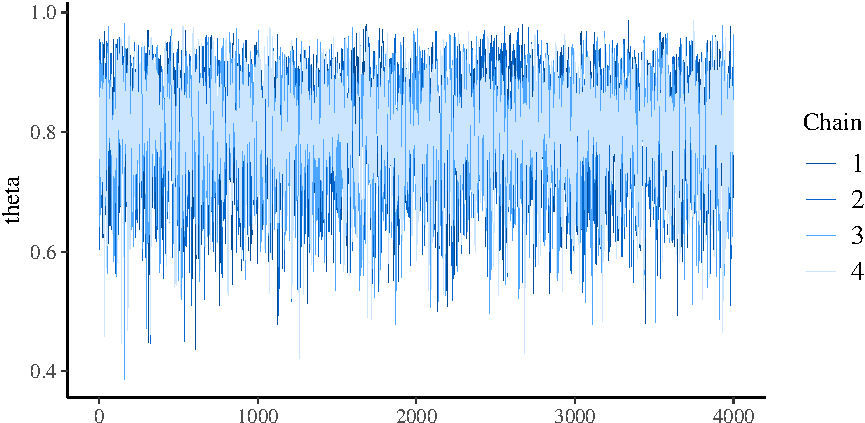
\includegraphics{040_modello_binomiale_files/figure-latex/trace-plot-gautret-1} 

}

\caption{Trace-plot per il parametro $\theta$ nel modello Beta-Binomiale.}\label{fig:trace-plot-gautret}
\end{figure}

\noindent
La figura \ref{fig:trace-plot-gautret} mostra che le catene esplorano uno spazio compreso approssimativamenre tra 0.7 e 0.9; tale figura descrive il comportamento \emph{longitudinale} delle catene di Markov.

Possiamo anche esaminare la distribuzione degli stati della catena di Markov, ovvero, dei valori che queste catene visitano lungo il loro percorso, ignorando l'ordine di queste visite. L'istogramma della figura \ref{fig:hist-post-gautret} fornisce una rappresentazione grafica di questa distribuzione per i 16000 valori complessivi delle quattro catene, ovvero per 4000 valori provienienti da ciascuna catena.

\begin{Shaded}
\begin{Highlighting}[]
\FunctionTok{mcmc\_hist}\NormalTok{(stanfit1, }\AttributeTok{pars =} \StringTok{"theta"}\NormalTok{) }\SpecialCharTok{+}
  \FunctionTok{yaxis\_text}\NormalTok{(}\ConstantTok{TRUE}\NormalTok{) }\SpecialCharTok{+}
  \FunctionTok{ylab}\NormalTok{(}\StringTok{"count"}\NormalTok{)}
\end{Highlighting}
\end{Shaded}

\begin{figure}

{\centering 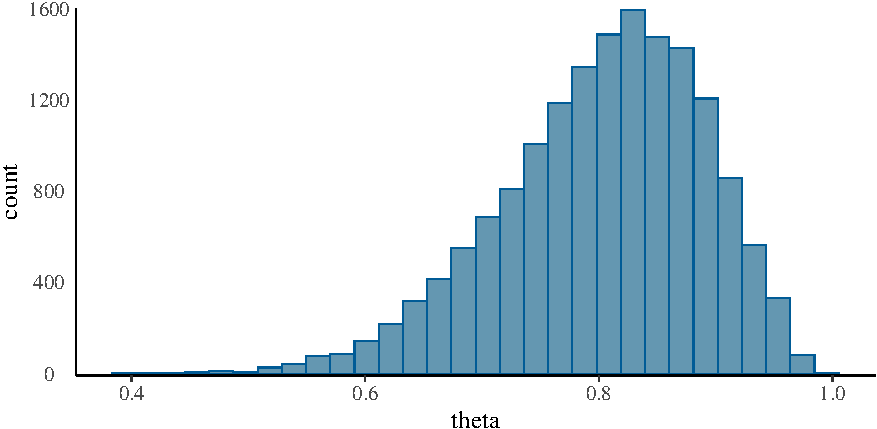
\includegraphics{040_modello_binomiale_files/figure-latex/hist-post-gautret-1} 

}

\caption{Istogramma che illustra l'approssimazione della distribuzione a posteriori per il parametro $\theta$ nel modello Beta-Binomiale.}\label{fig:hist-post-gautret}
\end{figure}

Nel modello Beta-Binomiale in cui la verosimiglianza è binomiale con 14 successi su 16 prove e in cui assumiamo una distribuzione a priori di tipo \(\mbox{Beta}(2, 2)\) sul parametro \(\theta\), la distribuzione a posteriori è ancora una distribuzione Beta di parametri \(\alpha\) = 2 + 14 e \(\beta\) = 2 + 16 - 14. La figura \ref{fig:hist-post-gautret-plus-correct} riporta un kernel density plot per i valori delle quattro catene di Markov con sovrapposta in nero la densità \(\mbox{Beta}(16, 4)\). Il punto importante è che la distribuzione dei valori delle catene di Markov produce un'eccellente approssimazione alla distribuzione bersaglio.\footnote{Nel caso presente, il risultato è poco utile dato che è disponibile una soluzione analitica. Tuttavia, questo esercizio mette in evidenza il fatto cruciale che, nei casi in cui possiamo verificarne la soluzione, il campionamento Monte Carlo a catena di Markov è in grado di trovare la risposta corretta. Di conseguenza, possiamo anche essere sicuri che fornirà un'approssimazione alla distribuzione a posteriori anche in quei casi in cui una soluzione analitica non è disponibile.}

\begin{Shaded}
\begin{Highlighting}[]
\FunctionTok{mcmc\_dens}\NormalTok{(stanfit1, }\AttributeTok{pars =} \StringTok{"theta"}\NormalTok{) }\SpecialCharTok{+}
  \FunctionTok{yaxis\_text}\NormalTok{(}\ConstantTok{TRUE}\NormalTok{) }\SpecialCharTok{+}
  \FunctionTok{ylab}\NormalTok{(}\StringTok{"density"}\NormalTok{) }\SpecialCharTok{+}
  \FunctionTok{stat\_function}\NormalTok{(}\AttributeTok{fun =}\NormalTok{ dbeta, }\AttributeTok{args =} \FunctionTok{list}\NormalTok{(}\AttributeTok{shape1 =} \DecValTok{16}\NormalTok{, }\AttributeTok{shape2 =} \DecValTok{4}\NormalTok{))}
\end{Highlighting}
\end{Shaded}

\begin{figure}

{\centering 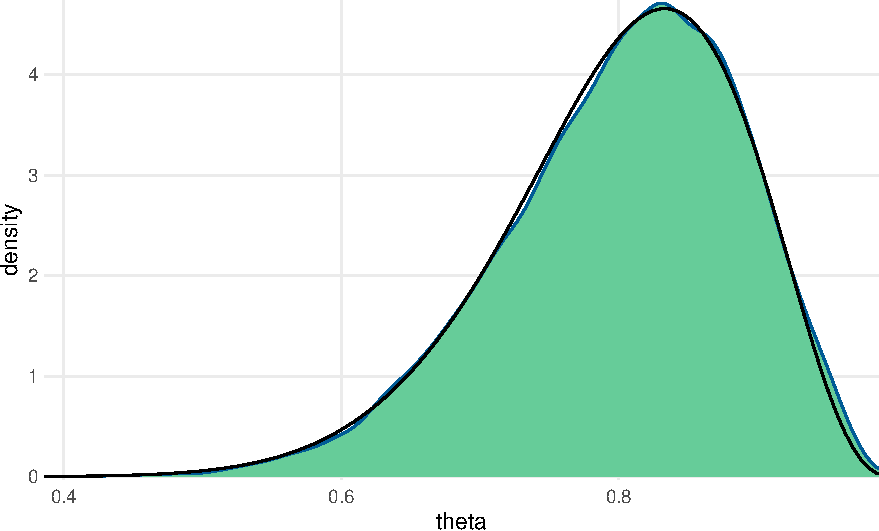
\includegraphics{040_modello_binomiale_files/figure-latex/hist-post-gautret-plus-correct-1} 

}

\caption{Istogramma che illustra l'approssimazione della distribuzione a posteriori per il parametro $\theta$ nel modello Beta-Binomiale. La curva nera rappresenta la corretta distribuzione a posteriori Beta(16, 4).}\label{fig:hist-post-gautret-plus-correct}
\end{figure}

Un intervallo di credibilità al 95\% per \(\theta\) si ottiene con la seguente chiamata:

\begin{Shaded}
\begin{Highlighting}[]
\NormalTok{posterior1 }\OtherTok{\textless{}{-}} \FunctionTok{extract}\NormalTok{(stanfit1)}
\NormalTok{rstantools}\SpecialCharTok{::}\FunctionTok{posterior\_interval}\NormalTok{(}\FunctionTok{as.matrix}\NormalTok{(stanfit1), }\AttributeTok{prob =} \FloatTok{0.95}\NormalTok{)}
\CommentTok{\#\textgreater{}                    2.5\%        97.5\%}
\CommentTok{\#\textgreater{} theta         0.6107860   0.94402990}
\CommentTok{\#\textgreater{} y\_rep[1]      0.0000000   1.00000000}
\CommentTok{\#\textgreater{} y\_rep[2]      0.0000000   1.00000000}
\CommentTok{\#\textgreater{} y\_rep[3]      0.0000000   1.00000000}
\CommentTok{\#\textgreater{} y\_rep[4]      0.0000000   1.00000000}
\CommentTok{\#\textgreater{} y\_rep[5]      0.0000000   1.00000000}
\CommentTok{\#\textgreater{} y\_rep[6]      0.0000000   1.00000000}
\CommentTok{\#\textgreater{} y\_rep[7]      0.0000000   1.00000000}
\CommentTok{\#\textgreater{} y\_rep[8]      0.0000000   1.00000000}
\CommentTok{\#\textgreater{} y\_rep[9]      0.0000000   1.00000000}
\CommentTok{\#\textgreater{} y\_rep[10]     0.0000000   1.00000000}
\CommentTok{\#\textgreater{} y\_rep[11]     0.0000000   1.00000000}
\CommentTok{\#\textgreater{} y\_rep[12]     0.0000000   1.00000000}
\CommentTok{\#\textgreater{} y\_rep[13]     0.0000000   1.00000000}
\CommentTok{\#\textgreater{} y\_rep[14]     0.0000000   1.00000000}
\CommentTok{\#\textgreater{} y\_rep[15]     0.0000000   1.00000000}
\CommentTok{\#\textgreater{} y\_rep[16]     0.0000000   1.00000000}
\CommentTok{\#\textgreater{} log\_lik[1]   {-}0.4930093  {-}0.05759735}
\CommentTok{\#\textgreater{} log\_lik[2]   {-}0.4930093  {-}0.05759735}
\CommentTok{\#\textgreater{} log\_lik[3]   {-}0.4930093  {-}0.05759735}
\CommentTok{\#\textgreater{} log\_lik[4]   {-}0.4930093  {-}0.05759735}
\CommentTok{\#\textgreater{} log\_lik[5]   {-}0.4930093  {-}0.05759735}
\CommentTok{\#\textgreater{} log\_lik[6]   {-}0.4930093  {-}0.05759735}
\CommentTok{\#\textgreater{} log\_lik[7]   {-}0.4930093  {-}0.05759735}
\CommentTok{\#\textgreater{} log\_lik[8]   {-}0.4930093  {-}0.05759735}
\CommentTok{\#\textgreater{} log\_lik[9]   {-}0.4930093  {-}0.05759735}
\CommentTok{\#\textgreater{} log\_lik[10]  {-}0.4930093  {-}0.05759735}
\CommentTok{\#\textgreater{} log\_lik[11]  {-}0.4930093  {-}0.05759735}
\CommentTok{\#\textgreater{} log\_lik[12]  {-}0.4930093  {-}0.05759735}
\CommentTok{\#\textgreater{} log\_lik[13]  {-}0.4930093  {-}0.05759735}
\CommentTok{\#\textgreater{} log\_lik[14]  {-}0.4930093  {-}0.05759735}
\CommentTok{\#\textgreater{} log\_lik[15]  {-}2.8829362  {-}0.94362543}
\CommentTok{\#\textgreater{} log\_lik[16]  {-}2.8829362  {-}0.94362543}
\CommentTok{\#\textgreater{} lp\_\_        {-}12.7342100 {-}10.00860000}
\end{Highlighting}
\end{Shaded}

Svolgendo un'analisi bayesiana simile a questa, \textcite{Gautret_2020} hanno trovato che gli intervalli di credibilità del gruppo di controllo e del gruppo sperimentale non si sovrappongono. Questo fatto viene interpretato dicendo che il parametro \(\theta\) è diverso nei due gruppi. Sulla base di queste evidenza, \textcite{Gautret_2020} hanno concluso, con un grado di certezza soggettiva del 95\%, che nel gruppo sperimentale vi è una probabilità più bassa di risultare positivi al SARS-CoV-2 rispetto al gruppo di controllo. In altri termini, questa analisi dei dati suggerisce che l'idrossiclorochina sia efficace come terapia per il Covid-19.

\hypertarget{la-critica-di-hulme_2020}{%
\subsection{\texorpdfstring{La critica di \textcite{Hulme_2020}}{La critica di @Hulme\_2020}}\label{la-critica-di-hulme_2020}}

Un articolo pubblicato da \textcite{Hulme_2020} si è posto il problema di rianalizzare i dati di \textcite{Gautret_2020}.\footnote{Si veda \url{https://osf.io/5dgmx/}.} Tra gli autori di questo articolo figura anche Eric-Jan Wagenmakers, uno psicologo molto conosciuto per i suoi contributi metodologici.
\textcite{Hulme_2020} hanno osservato che, nelle analisi statistiche riportate, \textcite{Gautret_2020} hanno escluso alcuni dati. Nel gruppo sperimentale, infatti, vi erano alcuni pazienti i quali, anziché migliorare, sono in realtà peggiorati. L'analisi statistica di \textcite{Gautret_2020} ha escluso i dati di questi pazienti.
Se consideriamo tutti i pazienti --- non solo quelli selezionati da \textcite{Gautret_2020} --- la situazione diventa la seguente:

\begin{itemize}
\tightlist
\item
  gruppo sperimentale: 10 positivi su 18;
\item
  gruppo di controllo: 14 positivi su 16.
\end{itemize}

L'analisi dei dati proposta da \textcite{Hulme_2020} richiede l'uso di alcuni strumenti statistici che, in queste dispense, non verranno discussi. Ma possiamo giungere alle stesse conclusioni raggiunte da questi ricercatori anche usando le procedure statistiche descritte nel Paragrafo successivo.

\hypertarget{due-proporzioni}{%
\section{Due proporzioni}\label{due-proporzioni}}

Svolgiamo ora l'analisi considerando tutti i dati, come suggerito da \textcite{Hulme_2020}. Per fare questo verrà creato un modello bayesiano per fare inferenza sulla differenza tra due proporzioni. Una volta generate le distribuzioni a posteriori per le proporzioni di ``successi'' nei due gruppi, verrà anche generata la quantità
\[
\omega = \frac{\theta_2 / (1-\theta_2)}{\theta_1 / (1-\theta_1)},
\]
\noindent
ovvero il rapporto tra gli Odds di positività tra i pazienti del gruppo di controllo e gli Odds di positività tra i pazienti del gruppo sperimentale. Se il valore dell'OR è uguale a 1, significa che l'Odds di positività nel gruppo di controllo è uguale all'odds di positività nel gruppo sperimentale, cioè il fattore in esame (somministrazione dell'idrossiclorochina) è ininfluente sulla comparsa della malattia. L'inferenza statistica sull'efficacia dell'idrossiclorochina come terapia per il Covid-19 può dunque essere effettuata esaminando l'intervallo di credibilità al 95\% per l'OR: se tale intervallo include il valore 1, allora non vi è evidenza che l'idrossiclorochina sia efficace come terapia per il Covid-19.

Nell'implementazione di questo modello, la quantità di interesse è dunque l'odds ratio; tale quantità viene calcolata nel blocco \texttt{generated\ quantities} del programma Stan. In questo esempio useremo delle distribuzioni a priori vagamente informative per i parametri \(\theta_1\) e \(\theta_1\).

\begin{Shaded}
\begin{Highlighting}[]
\NormalTok{data\_list }\OtherTok{\textless{}{-}} \FunctionTok{list}\NormalTok{(}
  \AttributeTok{N1 =} \DecValTok{18}\NormalTok{,}
  \AttributeTok{y1 =} \DecValTok{10}\NormalTok{,}
  \AttributeTok{N2 =} \DecValTok{16}\NormalTok{,}
  \AttributeTok{y2 =} \DecValTok{14}
\NormalTok{)}
\end{Highlighting}
\end{Shaded}

\begin{Shaded}
\begin{Highlighting}[]
\NormalTok{modelString }\OtherTok{\textless{}{-}} \StringTok{"}
\StringTok{//  Comparison of two groups with Binomial}
\StringTok{data \{}
\StringTok{  int\textless{}lower=0\textgreater{} N1;              // number of experiments in group 1}
\StringTok{  int\textless{}lower=0\textgreater{} y1;              // number of deaths in group 1}
\StringTok{  int\textless{}lower=0\textgreater{} N2;              // number of experiments in group 2}
\StringTok{  int\textless{}lower=0\textgreater{} y2;              // number of deaths in group 2}
\StringTok{\}}
\StringTok{parameters \{}
\StringTok{  real\textless{}lower=0,upper=1\textgreater{} theta1; // probability of death in group 1}
\StringTok{  real\textless{}lower=0,upper=1\textgreater{} theta2; // probability of death in group 2}
\StringTok{\}}
\StringTok{model \{}
\StringTok{  theta1 \textasciitilde{} beta(2, 2);          // prior}
\StringTok{  theta2 \textasciitilde{} beta(2, 2);          // prior}
\StringTok{  y1 \textasciitilde{} binomial(N1, theta1);    // observation model / likelihood}
\StringTok{  y2 \textasciitilde{} binomial(N2, theta2);    // observation model / likelihood}
\StringTok{\}}
\StringTok{generated quantities \{}
\StringTok{  // generated quantities are computed after sampling}
\StringTok{  real oddsratio = (theta2/(1{-}theta2))/(theta1/(1{-}theta1));}
\StringTok{\}}
\StringTok{"}
\FunctionTok{writeLines}\NormalTok{(modelString, }\AttributeTok{con =} \StringTok{"code/twoprop1.stan"}\NormalTok{)}
\end{Highlighting}
\end{Shaded}

\begin{Shaded}
\begin{Highlighting}[]
\NormalTok{file }\OtherTok{\textless{}{-}} \FunctionTok{file.path}\NormalTok{(}\StringTok{"code"}\NormalTok{, }\StringTok{"twoprop1.stan"}\NormalTok{)}
\end{Highlighting}
\end{Shaded}

\begin{Shaded}
\begin{Highlighting}[]
\NormalTok{mod }\OtherTok{\textless{}{-}} \FunctionTok{cmdstan\_model}\NormalTok{(file)}
\end{Highlighting}
\end{Shaded}

\begin{Shaded}
\begin{Highlighting}[]
\NormalTok{fit }\OtherTok{\textless{}{-}}\NormalTok{ mod}\SpecialCharTok{$}\FunctionTok{sample}\NormalTok{(}
  \AttributeTok{data =}\NormalTok{ data\_list,}
  \AttributeTok{iter\_sampling =}\NormalTok{ 4000L,}
  \AttributeTok{iter\_warmup =}\NormalTok{ 2000L,}
  \AttributeTok{seed =}\NormalTok{ SEED,}
  \AttributeTok{chains =}\NormalTok{ 4L,}
  \AttributeTok{parallel\_chains =}\NormalTok{ 4L,}
  \AttributeTok{refresh =} \DecValTok{0}\NormalTok{,}
  \AttributeTok{thin =} \DecValTok{1}
\NormalTok{)}
\end{Highlighting}
\end{Shaded}

\begin{Shaded}
\begin{Highlighting}[]
\NormalTok{stanfit }\OtherTok{\textless{}{-}}\NormalTok{ rstan}\SpecialCharTok{::}\FunctionTok{read\_stan\_csv}\NormalTok{(fit}\SpecialCharTok{$}\FunctionTok{output\_files}\NormalTok{())}
\end{Highlighting}
\end{Shaded}

\begin{Shaded}
\begin{Highlighting}[]
\FunctionTok{print}\NormalTok{(}
\NormalTok{  stanfit,}
  \AttributeTok{pars =} \FunctionTok{c}\NormalTok{(}\StringTok{"theta1"}\NormalTok{, }\StringTok{"theta2"}\NormalTok{, }\StringTok{"oddsratio"}\NormalTok{),}
  \AttributeTok{digits\_summary =}\NormalTok{ 3L}
\NormalTok{)}
\CommentTok{\#\textgreater{} Inference for Stan model: twoprop1{-}202110161322{-}1{-}604a8b.}
\CommentTok{\#\textgreater{} 4 chains, each with iter=6000; warmup=2000; thin=1; }
\CommentTok{\#\textgreater{} post{-}warmup draws per chain=4000, total post{-}warmup draws=16000.}
\CommentTok{\#\textgreater{} }
\CommentTok{\#\textgreater{}            mean se\_mean    sd  2.5\%   25\%   50\%   75\%}
\CommentTok{\#\textgreater{} theta1    0.546   0.001 0.104 0.337 0.475 0.547 0.619}
\CommentTok{\#\textgreater{} theta2    0.801   0.001 0.087 0.605 0.747 0.812 0.865}
\CommentTok{\#\textgreater{} oddsratio 4.859   0.049 4.740 0.914 2.221 3.599 5.933}
\CommentTok{\#\textgreater{}            97.5\% n\_eff  Rhat}
\CommentTok{\#\textgreater{} theta1     0.743 11214 1.000}
\CommentTok{\#\textgreater{} theta2     0.939 12359 1.000}
\CommentTok{\#\textgreater{} oddsratio 16.251  9207 1.001}
\CommentTok{\#\textgreater{} }
\CommentTok{\#\textgreater{} Samples were drawn using NUTS(diag\_e) at Sab Ott 16 13:22:40 2021.}
\CommentTok{\#\textgreater{} For each parameter, n\_eff is a crude measure of effective sample size,}
\CommentTok{\#\textgreater{} and Rhat is the potential scale reduction factor on split chains (at }
\CommentTok{\#\textgreater{} convergence, Rhat=1).}
\end{Highlighting}
\end{Shaded}

L'intervallo di credibilità del 95\% per l'OR include il valore di 1.0 (ovvero, il valore che indica che gli odds di positività sono uguali nei due gruppi). In base agli standard correnti, un risultato di questo tipo non viene considerato come evidenza sufficiente per potere concludere che il parametro \(\theta\) assume un valore diverso nei due gruppi. In altri termini, se consideriamo tutti i dati, e non solo quelli selezionati dagli autori della ricerca originaria, non vi è evidenza alcuna che l'idrossiclorochina sia efficace come terapia per il Covid-19.

\hypertarget{considerazioni-conclusive}{%
\section*{Considerazioni conclusive}\label{considerazioni-conclusive}}
\addcontentsline{toc}{section}{Considerazioni conclusive}

Concludiamo questa discussione dicendo che ciò che è stato presentato in questo capitolo è un esercizio didattico: la ricerca di \textcite{Gautret_2020} include tante altre informazioni che non sono state qui considerate. Tuttavia, notiamo che la semplice analisi statistica che abbiamo qui descritto è stata in grado di replicare le conclusioni a cui sono giunti (per altra via) \textcite{Hulme_2020}.

\hypertarget{diagn-markov-chains}{%
\chapter{Diagnostica delle catene markoviane}\label{diagn-markov-chains}}

Come discusso nel Paragrafo \ref{cmdstanr-gautret}, le catene di Markov forniscono un'approssimazione che tende a convergere alla distribuzione a posteriori. ``Approssimazione'' e ``convergenza'' sono le parole chiave qui: il punto è che il campionamento MCMC non è perfetto. Questo solleva le seguenti domande:

\begin{itemize}
\tightlist
\item
  A cosa corrisponde, dal punto di vista grafico, una ``buona'' catena di Markov?
\item
  Come possiamo sapere se il campione prodotto dalla catena di Markov costituisce un'approssimazione adeguata della distribuzione a posteriori?
\item
  Quanto deve essere grande la dimensione del campione casuale prodotto dalla catena Markov?
\end{itemize}

Rispondere a queste ed altre domande di questo tipo fa parte di quell'insieme di pratiche che vano sotto il nome di \emph{diagnostica delle catene Markoviane}.

La diagnostica delle catene Markoviane non è ``una scienza esatta''. Ovvero, non sono disponibili procedure valide in tutti i casi e non sempre siamo in grado di rispondere alle domande precedenti. È piuttosto l'esperienza del ricercatore che consente di riconoscere una ``buona'' catena di Markov e a suggerire cosa si può fare per riparare una ``cattiva'' catena di Markov. In questo Capitolo ci concentreremo su alcuni strumenti diagnostici grafici e numerici che possono essere utilizzati per la diagnostica delle catene markoviane. L'utilizzo di questi strumenti diagnostici deve essere eseguito in modo olistico. Nessuna singola diagnostica visiva o numerica è infatti sufficiente: un quadro completo della qualità della catena di Markov si può solo ottenere considerando tutti gli strumenti descritti di seguito.

\hypertarget{esame-dei-trace-plot}{%
\section{\texorpdfstring{Esame dei \emph{trace plot}}{Esame dei trace plot}}\label{esame-dei-trace-plot}}

La convergenza e il ``mixing'' possono essere controllate mediante il \emph{trace plot} che mostra l'andamento delle simulazioni e ci dice se stiamo effettivamente utilizzando una distribuzione limite. Consideriamo nuovamente il \emph{trace plot} del simulazione Beta-Binomiale della figura \ref{fig:trace-plot-gautret-2}:

\begin{figure}

{\centering 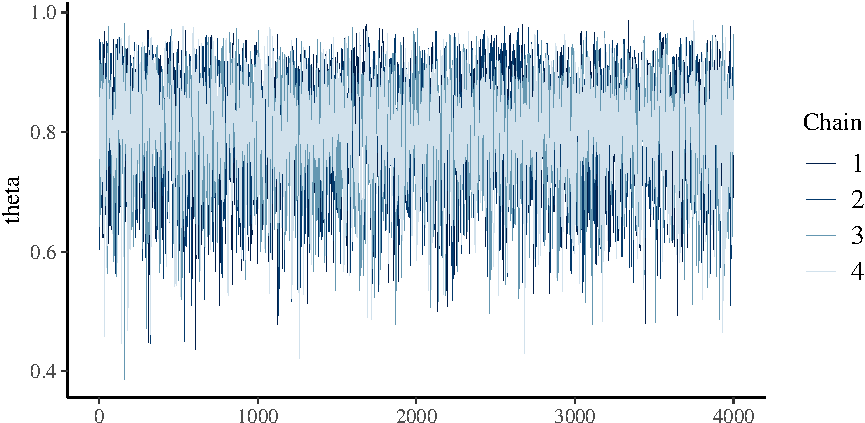
\includegraphics{041_diagnostica_MCMC_files/figure-latex/trace-plot-gautret-2-1} 

}

\caption{Trace plot per il modello Beta-Binomiale dei dati di Gautret et al.(2020).}\label{fig:trace-plot-gautret-2}
\end{figure}

La figura \ref{fig:trace-plot-gautret-2} fornisce un esempio perfetto di come dovrebbero apparire i \emph{trace plot}. Quando le catene markoviane raggiungono uno stato stazionario e sono stabili ciò significa che hanno raggiunto la distribuzione stazionaria e il \emph{trace plot} rivela una assenza di struttura e assomiglia alla rappresentazione del rumore bianco, come nella figura \ref{fig:trace-plot-gautret-2}.
Al contrario, la figura \ref{fig:bad-trace-bayesrules} indica mancanza di convergenza\footnote{Figura riprodotta da \textcite{Johnson2022bayesrules}}.

\begin{figure}

{\centering 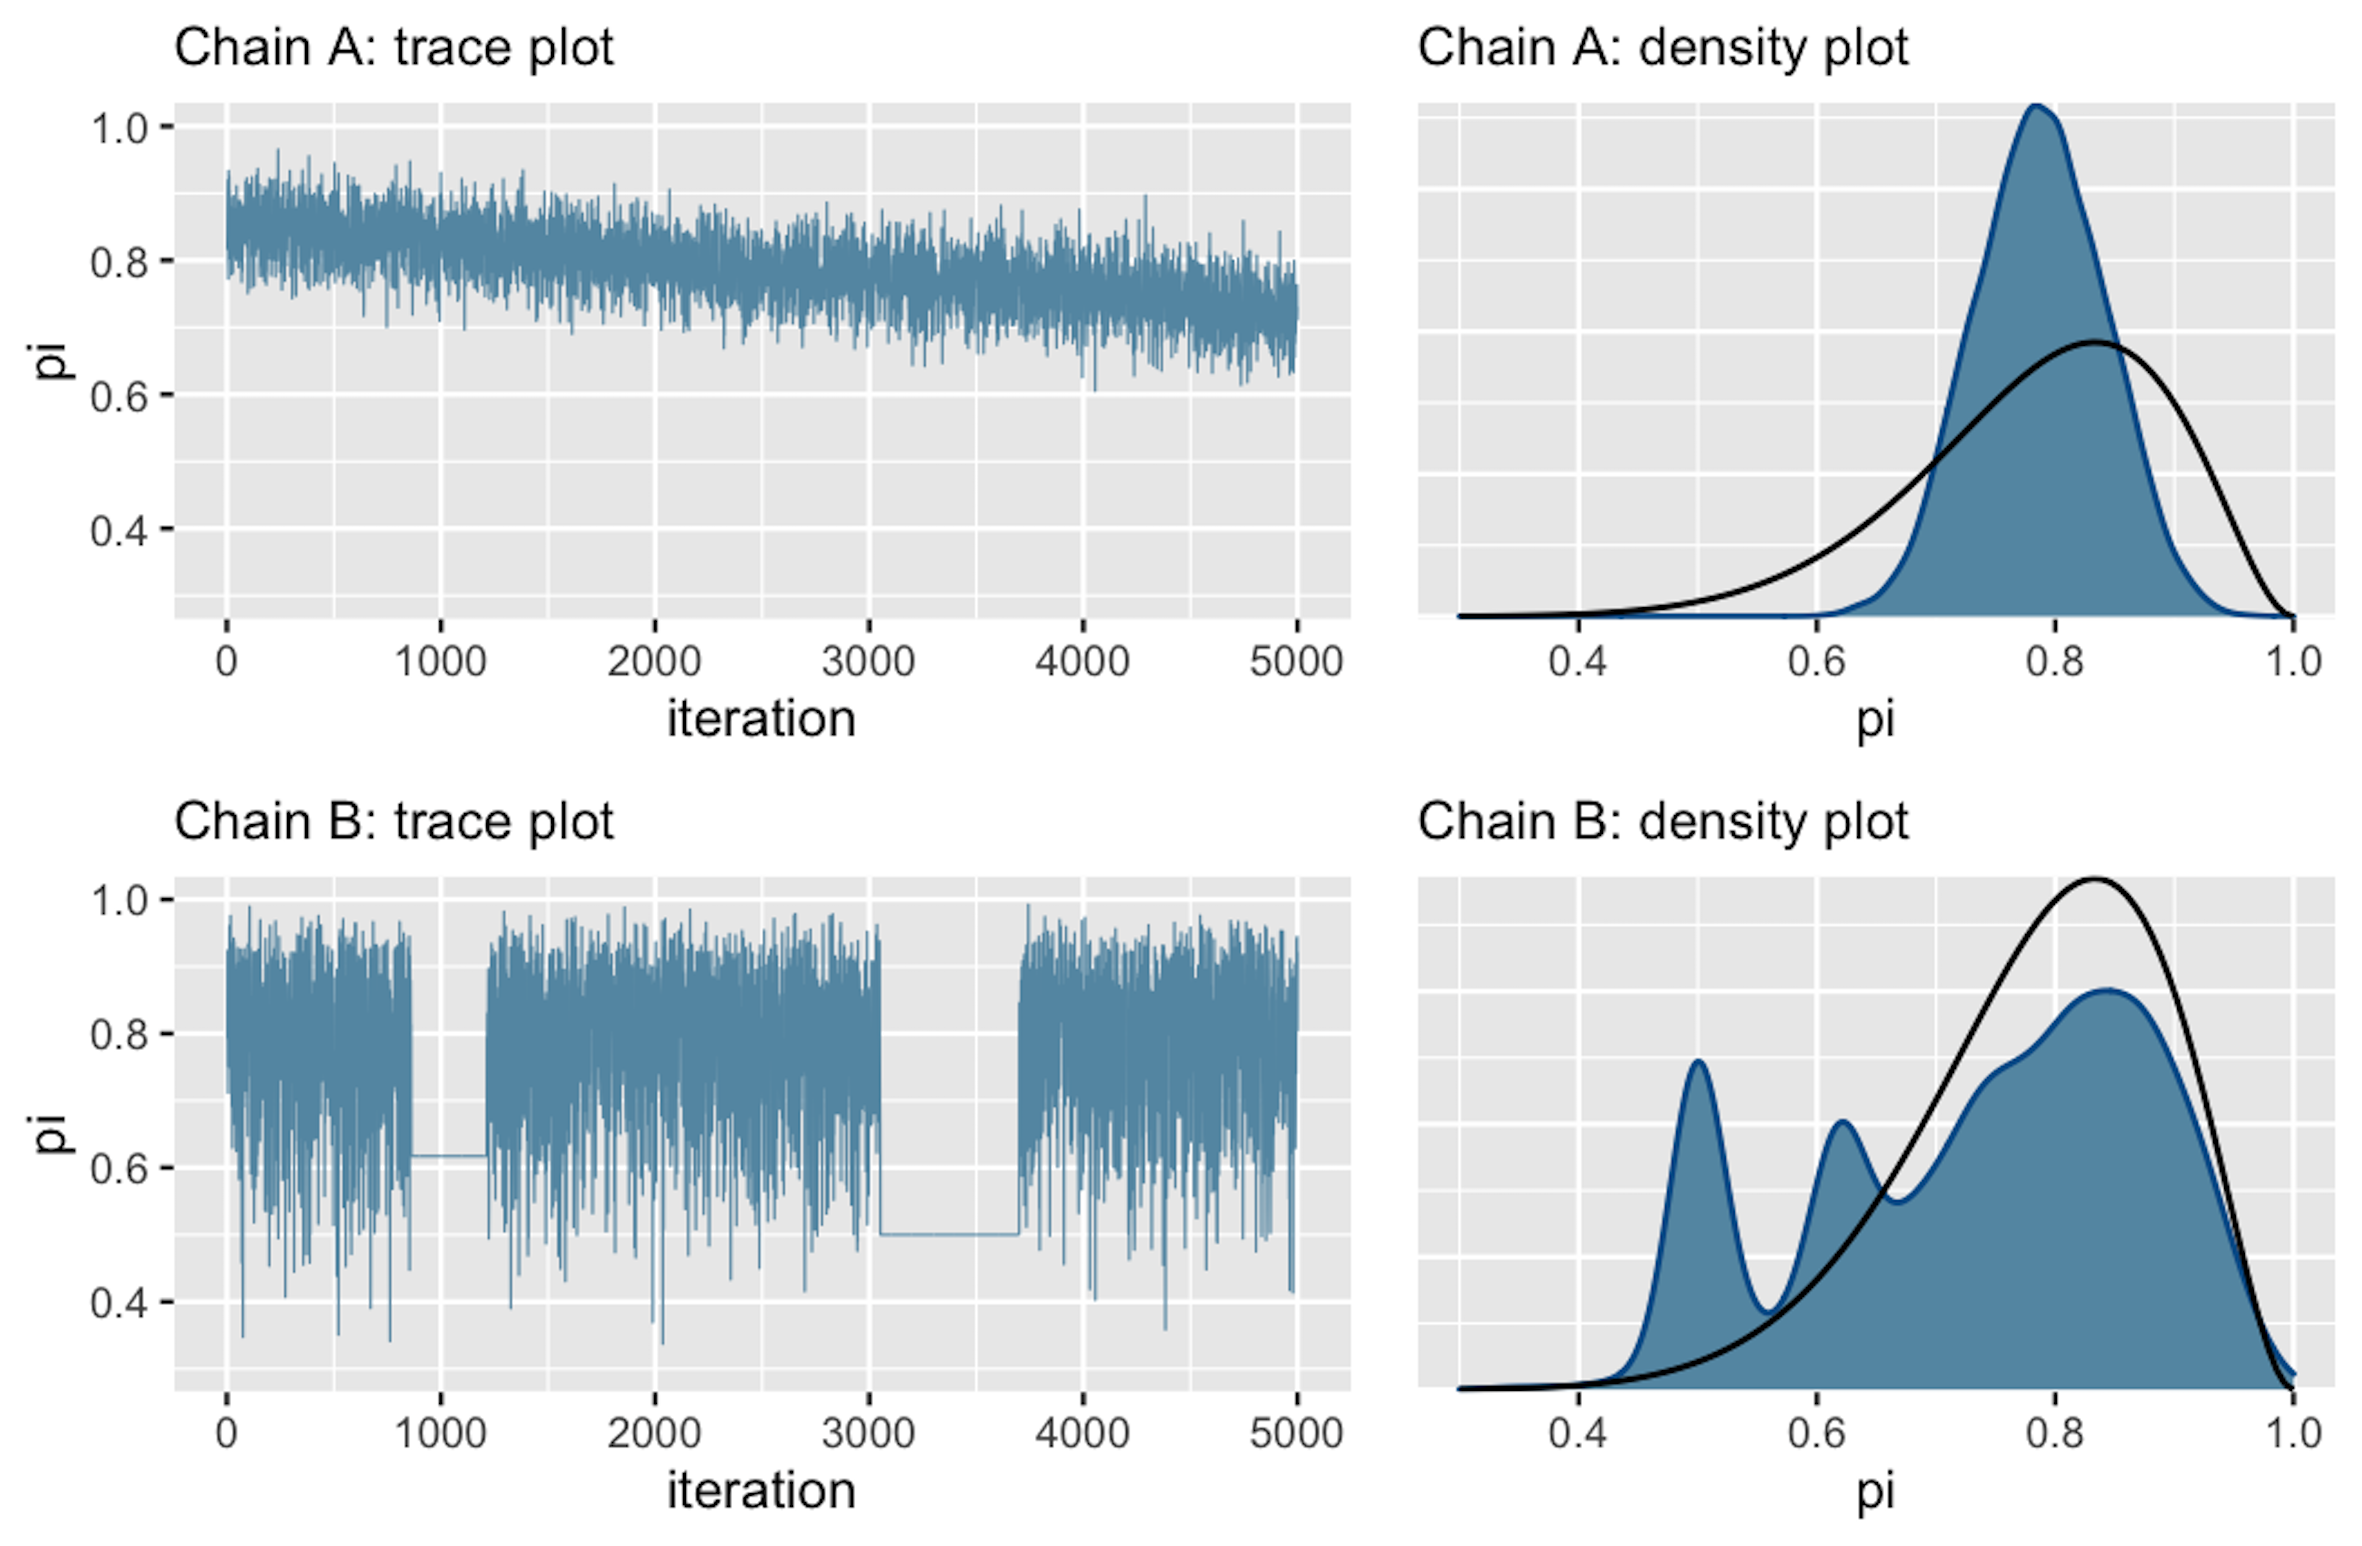
\includegraphics[width=32.81in]{images/bad-trace-bayesrules} 

}

\caption{Trace plots (a sinistra) e corrispondenti grafici di densità (a destra) di due ipotetiche catene di Markov. Queste figure forniscono due esempi di come potrebbero apparire delle catene di Markov non stazionarie. Le linee nere sovrapposte alle densità empiriche (a destra) rappresentano una ipotetica distribuzione target Beta(11,3).}\label{fig:bad-trace-bayesrules}
\end{figure}

Consideriamo i trace-plot della figura \ref{fig:bad-trace-bayesrules} (a sinistra). La tendenza verso il basso indica che la catena A non è stazionaria, ovvero non si mantiene costante all'evolversi nel tempo. La tendenza verso il basso suggerisce inoltre la presenza di una forte correlazione tra i valori della catena: il trace-plot non fornisce una rappresentazione di rumore indipendente. Tutto questo significa che la catena A ``si sta mescolando lentamente''. Sebbene le catene di Markov siano intrinsecamente dipendenti, più si comportano come se fossero dei campioni casuali (rumorosi), minore è l'errore dell'approssimazione alla distribuzione a posteriori. La catena B presenta un problema diverso. Come evidenziato dalle due linee completamente piatte nel tracciato, essa tende a bloccarsi quando visita valori bassi di \(\theta\).

Gli istogrammi lisciati della figura \ref{fig:bad-trace-bayesrules} (a destra) confermano che entrambe queste catene sono problematiche: infatti producono approssimazioni scadenti della distribuzione a posteriori che, nell'esempio di \textcite{Johnson2022bayesrules}, è una \(\mbox{Beta}(11, 3)\) (curva nera nella figura). Consideriamo la catena A. Dal momento che si sta mescolando lentamente, nelle iterazioni eseguite ha esplorato unicamente i valori \(\theta\) nell'intervallo da 0.6 a 0.9. Di conseguenza, la sua approssimazione della distribuzione a posteriori sopravvaluta la plausibilità dei valori \(\theta\) in questo intervallo e, nel contempo, sottovaluta la plausibilità dei valori \(\theta\) esterni a questo intervallo. Consideriamo ora la catena B. Rimanendo bloccata, la catena B campiona in maniera eccessiva alcuni valori nella coda sinistra della distribuzione a posteriori di \(\theta\). Questo fenomeno produce i picchi che sono presenti nell'approssimazione alla distribuzione a posteriori.

In pratica, al di là dei presenti esempi ``scolastici'' (in cui disponiamo di una formulazione analitica della distribuzione a posteriori), non abbiamo mai il privilegio di poter confrontare i risultati del campionamento MCMC con la corretta distribuzione a posteriori. Ecco perché la diagnostica delle catene di Markov è così importante: se vediamo trace-plots come quelli della figura \ref{fig:bad-trace-bayesrules}, sappiamo che non abbiamo ottenuto una adeguata approssimazione della distribuzione a posteriori.

In tali circostanze possiamo ricorrere ad alcuni rimedi.

\begin{enumerate}
\def\labelenumi{\arabic{enumi}.}
\item
  Controllare il modello. Siamo sicuri che le distribuzioni a priori e la verosimiglianza siano appropriate per i dati osservati?
\item
  Utilizzare un numero maggiore di iterazioni. Alcune tendenze indesiderate a breve termine della catena possono appianarsi nel lungo termine.
\end{enumerate}

\hypertarget{confronto-delle-catene-parallele}{%
\section{Confronto delle catene parallele}\label{confronto-delle-catene-parallele}}

Nella simulazione \texttt{cmdstanr()} per il modello Beta-Binomiale dei dati di \textcite{Gautret_2020} abbiamo utilizzato quattro catene di Markov parallele. Non solo è necessario che ogni singola catena sia stazionaria (come discusso sopra), ma è anche necessario che le quattro catene siano coerenti tra loro. Sebbene le catene esplorino percorsi diversi nello spazio dei parametri, quando convergono ad uno stato di equilibrio dovrebbero presentare caratteristiche simili e dovrebbero produrre approssimazioni simili alla distribuzione a posteriori. Per l'esempio del modello Beta-Binomiale dei dati di \textcite{Gautret_2020}, i seguenti istogrammi lisciati indicano che le quattro catene producono approssimazioni quasi indistinguibili della distribuzione a posteriori. Ciò prova che la simulazione è stabile e contiene un nunero sufficiente di valori: l'esecuzione delle catene per un numero maggiore di iterazioni non migliorerebbe l'approssimazione della distribuzione a posteriori.

\begin{Shaded}
\begin{Highlighting}[]
\FunctionTok{mcmc\_dens\_overlay}\NormalTok{(stanfit1, }\AttributeTok{pars =} \StringTok{"theta"}\NormalTok{) }\SpecialCharTok{+}
  \FunctionTok{ylab}\NormalTok{(}\StringTok{"density"}\NormalTok{)}
\end{Highlighting}
\end{Shaded}

\begin{center}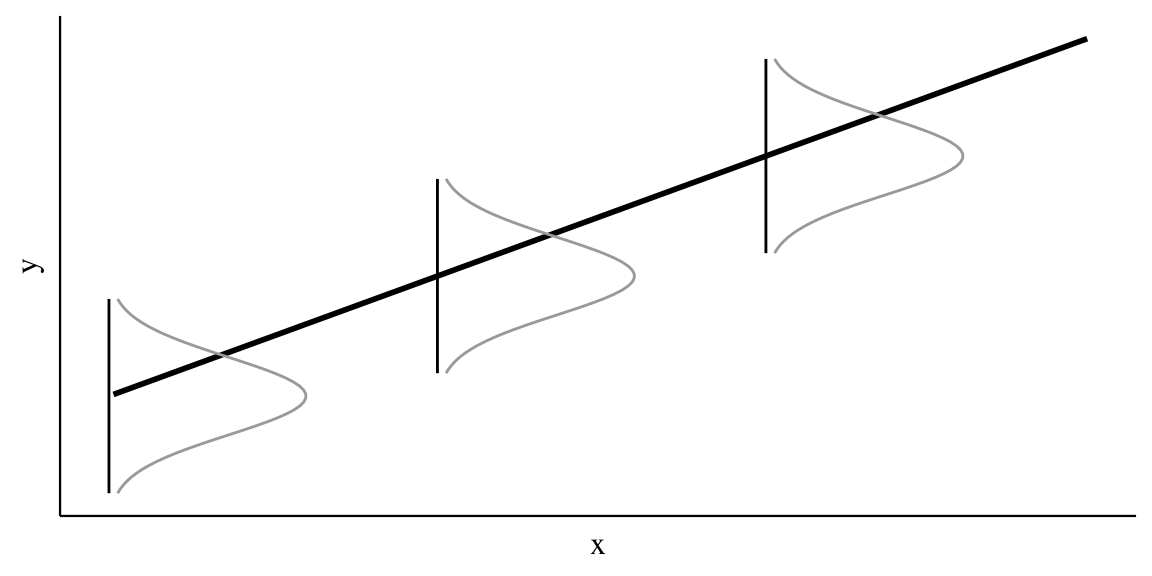
\includegraphics{041_diagnostica_MCMC_files/figure-latex/unnamed-chunk-2-1} \end{center}

Per fare un confronto, consideriamo la simulazione di una catena di Markov più corta per lo stesso modello. La chiamata seguente richiede quattro catene parallele per sole 100 iterazioni ciascuna:

\begin{Shaded}
\begin{Highlighting}[]
\NormalTok{bb\_short }\OtherTok{\textless{}{-}}\NormalTok{ mod}\SpecialCharTok{$}\FunctionTok{sample}\NormalTok{(}
  \AttributeTok{data =}\NormalTok{ data1\_list,}
  \AttributeTok{iter\_sampling =} \DecValTok{50} \SpecialCharTok{*}\NormalTok{ 2L,}
  \AttributeTok{seed =}\NormalTok{ SEED,}
  \AttributeTok{chains =}\NormalTok{ 4L,}
  \AttributeTok{parallel\_chains =}\NormalTok{ 4L,}
  \AttributeTok{refresh =} \DecValTok{0}\NormalTok{,}
  \AttributeTok{thin =} \DecValTok{1}
\NormalTok{)}
\ConstantTok{FALSE}\NormalTok{ Running MCMC with }\DecValTok{4}\NormalTok{ parallel chains...}
\ConstantTok{FALSE} 
\ConstantTok{FALSE}\NormalTok{ Chain }\DecValTok{1}\NormalTok{ finished }\ControlFlowTok{in} \FloatTok{0.0}\NormalTok{ seconds.}
\ConstantTok{FALSE}\NormalTok{ Chain }\DecValTok{2}\NormalTok{ finished }\ControlFlowTok{in} \FloatTok{0.0}\NormalTok{ seconds.}
\ConstantTok{FALSE}\NormalTok{ Chain }\DecValTok{3}\NormalTok{ finished }\ControlFlowTok{in} \FloatTok{0.0}\NormalTok{ seconds.}
\ConstantTok{FALSE}\NormalTok{ Chain }\DecValTok{4}\NormalTok{ finished }\ControlFlowTok{in} \FloatTok{0.0}\NormalTok{ seconds.}
\ConstantTok{FALSE} 
\ConstantTok{FALSE}\NormalTok{ All }\DecValTok{4}\NormalTok{ chains finished successfully.}
\ConstantTok{FALSE}\NormalTok{ Mean chain execution time}\SpecialCharTok{:} \FloatTok{0.0}\NormalTok{ seconds.}
\ConstantTok{FALSE}\NormalTok{ Total execution time}\SpecialCharTok{:} \FloatTok{0.2}\NormalTok{ seconds.}

\NormalTok{stanfit\_bb\_short }\OtherTok{\textless{}{-}}\NormalTok{ rstan}\SpecialCharTok{::}\FunctionTok{read\_stan\_csv}\NormalTok{(bb\_short}\SpecialCharTok{$}\FunctionTok{output\_files}\NormalTok{())}
\end{Highlighting}
\end{Shaded}

\noindent
Di seguito sono riportati i \emph{trace-plot} e i corrispondenti istogrammi lisciati.

\begin{Shaded}
\begin{Highlighting}[]
\FunctionTok{mcmc\_trace}\NormalTok{(stanfit\_bb\_short, }\AttributeTok{pars =} \StringTok{"theta"}\NormalTok{)}
\end{Highlighting}
\end{Shaded}

\begin{center}\includegraphics{041_diagnostica_MCMC_files/figure-latex/unnamed-chunk-4-1} \end{center}

\begin{Shaded}
\begin{Highlighting}[]
\FunctionTok{mcmc\_dens\_overlay}\NormalTok{(stanfit\_bb\_short, }\AttributeTok{pars =} \StringTok{"theta"}\NormalTok{)}
\end{Highlighting}
\end{Shaded}

\begin{center}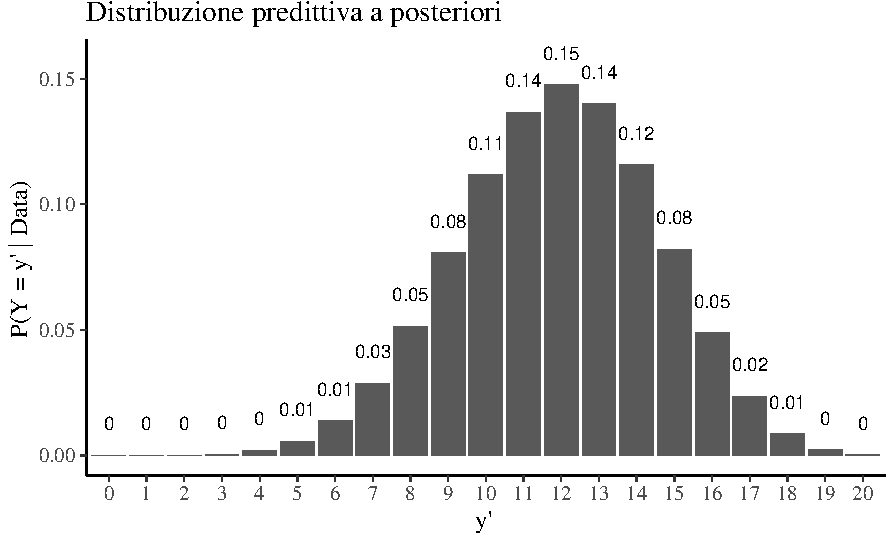
\includegraphics{041_diagnostica_MCMC_files/figure-latex/unnamed-chunk-5-1} \end{center}

Anche se i \emph{trace plot} sembrano tutti mostrare un andamento casuale, gli istogrammi lisciati sono piuttosto diversi tra loro e producono approssimazioni diverse della distribuzione a posteriori. Di fronte a tale instabilità è chiaro che sarebbe un errore interrompere la simulazione dopo solo 100 iterazioni.

\hypertarget{numerosita-campionaria-effettiva}{%
\section{Numerosità campionaria effettiva}\label{numerosita-campionaria-effettiva}}

Nella simulazione del modello Beta-Binomiale per i dati di \textcite{Gautret_2020} abbiamo utilizzato quattro catene di Markov parallele che producono un totale di \(N\) = 16000 campioni \emph{dipendenti} di \(\theta\). Sapendo che l'errore dell'approssimazione alla distribuzione a posteriori è probabilmente più grande di quello che si otterrebbe usando 16000 campioni \emph{indipendenti}, ci possiamo porre la seguente domanda: quanti campioni indipendenti sarebbero necessari per produrre un'approssimazione della distribuzione a posteriori equivalentemente a quella che abbiamo ottenuto? La numerosità campionaria effettiva (\emph{effective sample size}, \(N_{eff}\)) fornisce una risposta a questa domanda.

Tipicamente, \(N_{eff} < N\), per cui il rapporto campionario effettivo (\emph{effective sample size ratio}) \(\frac{N_{eff}}{N}\) è minore di 1. Come regola euristica, viene considerato problematico un rapporto campionario effettivo minore del 10\% del numero totale di campioni ottenuti nella simulazione (più basso è il rapporto campionario effettivo peggiore è il ``mixing'' della catena). La funzione \texttt{bayesplot::neff\_ratio()} consente di calcolare il rapporto campionario effettivo. Per il modello Beta-Binomiale dei dati di \textcite{Gautret_2020}, questo rapporto è di circa 0.34:

\begin{Shaded}
\begin{Highlighting}[]
\NormalTok{bayesplot}\SpecialCharTok{::}\FunctionTok{neff\_ratio}\NormalTok{(stanfit1, }\AttributeTok{pars =} \FunctionTok{c}\NormalTok{(}\StringTok{"theta"}\NormalTok{))}
\CommentTok{\#\textgreater{} [1] 0.3352141}
\end{Highlighting}
\end{Shaded}

Ciò indica che l'accuratezza dell'approssimazione della distribuzione a posteriori di \(\theta\) ottenuta mediante 16000 campioni dipendenti è approssimativamente simile a quella che si potrebbe ottenere con

\begin{Shaded}
\begin{Highlighting}[]
\NormalTok{bayesplot}\SpecialCharTok{::}\FunctionTok{neff\_ratio}\NormalTok{(stanfit1, }\AttributeTok{pars =} \FunctionTok{c}\NormalTok{(}\StringTok{"theta"}\NormalTok{)) }\SpecialCharTok{*} \DecValTok{16000}
\CommentTok{\#\textgreater{} [1] 5363.426}
\end{Highlighting}
\end{Shaded}

\noindent
campioni \emph{indipendenti}. In questo esempio, il rapporto campionario effettivo è maggiore di 0.1; dunque non ci sono problemi.

\hypertarget{autocorrelazione}{%
\section{Autocorrelazione}\label{autocorrelazione}}

Normalmente un algoritmo MCMC genera catene di Markov di campioni, ognuno dei quali è autocorrelato a quelli generati immediatamente prima e dopo di lui. Conseguentemente campioni successivi non sono indipendenti ma formano una catena di Markov con un certo grado di correlazione. Il valore \(\theta^{(i)}\) tende ad essere più simile al valore \(\theta^{(i-1)}\) che al valore \(\theta^{(i-2)}\), o al valore \(\theta^{(i-3)}\), eccetera. Una misura di ciò è fornita dall'autocorrelazione tra i valori consecutivi della catena.

Il correlogramma per ciascuna delle quattro catene dell'esempio si produce con la seguente chiamata:

\begin{Shaded}
\begin{Highlighting}[]
\NormalTok{bayesplot}\SpecialCharTok{::}\FunctionTok{mcmc\_acf}\NormalTok{(stanfit1, }\AttributeTok{pars =} \StringTok{"theta"}\NormalTok{)}
\end{Highlighting}
\end{Shaded}

\begin{center}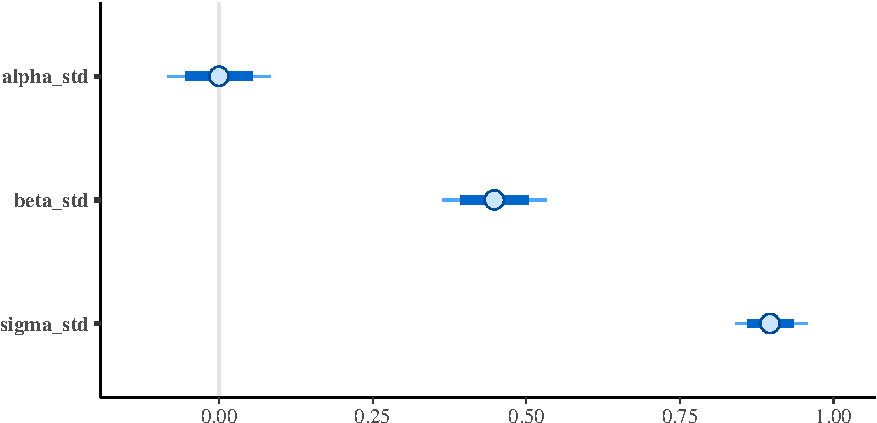
\includegraphics{041_diagnostica_MCMC_files/figure-latex/unnamed-chunk-8-1} \end{center}

Il correlogramma mostra l'autocorrelazione in funzione di ritardi da 0 a 20. L'autocorrelazione di lag 0 è naturalmente 1 -- misura la correlazione tra un valore della catena di Markov e se stesso. L'autocorrelazione di lag 1 è di circa 0.5, indicando una correlazione moderata tra i valori della catena che distano di solo 1 passo l'uno dall'altro. Successivamente, l'autocorrelazione diminuisce rapidamente ed è effettivamente pari a 0 per un lag di 5. Questo risultato fornisce una conferma del fatto che la catena di Markov costituisce una buona approssimazione di un campione casuale di \(p(\theta \mid y)\).

Al contrario, nella figura \ref{fig:bad-autocorrelation} (a destra) \autocite[riprodotta da][]{Johnson2022bayesrules} vediamo un esempio nel quale il trace plot rivela una forte tendenza tra i valori di una catena di Markov e, dunque, una forte autocorrelazione.

\begin{figure}

{\centering 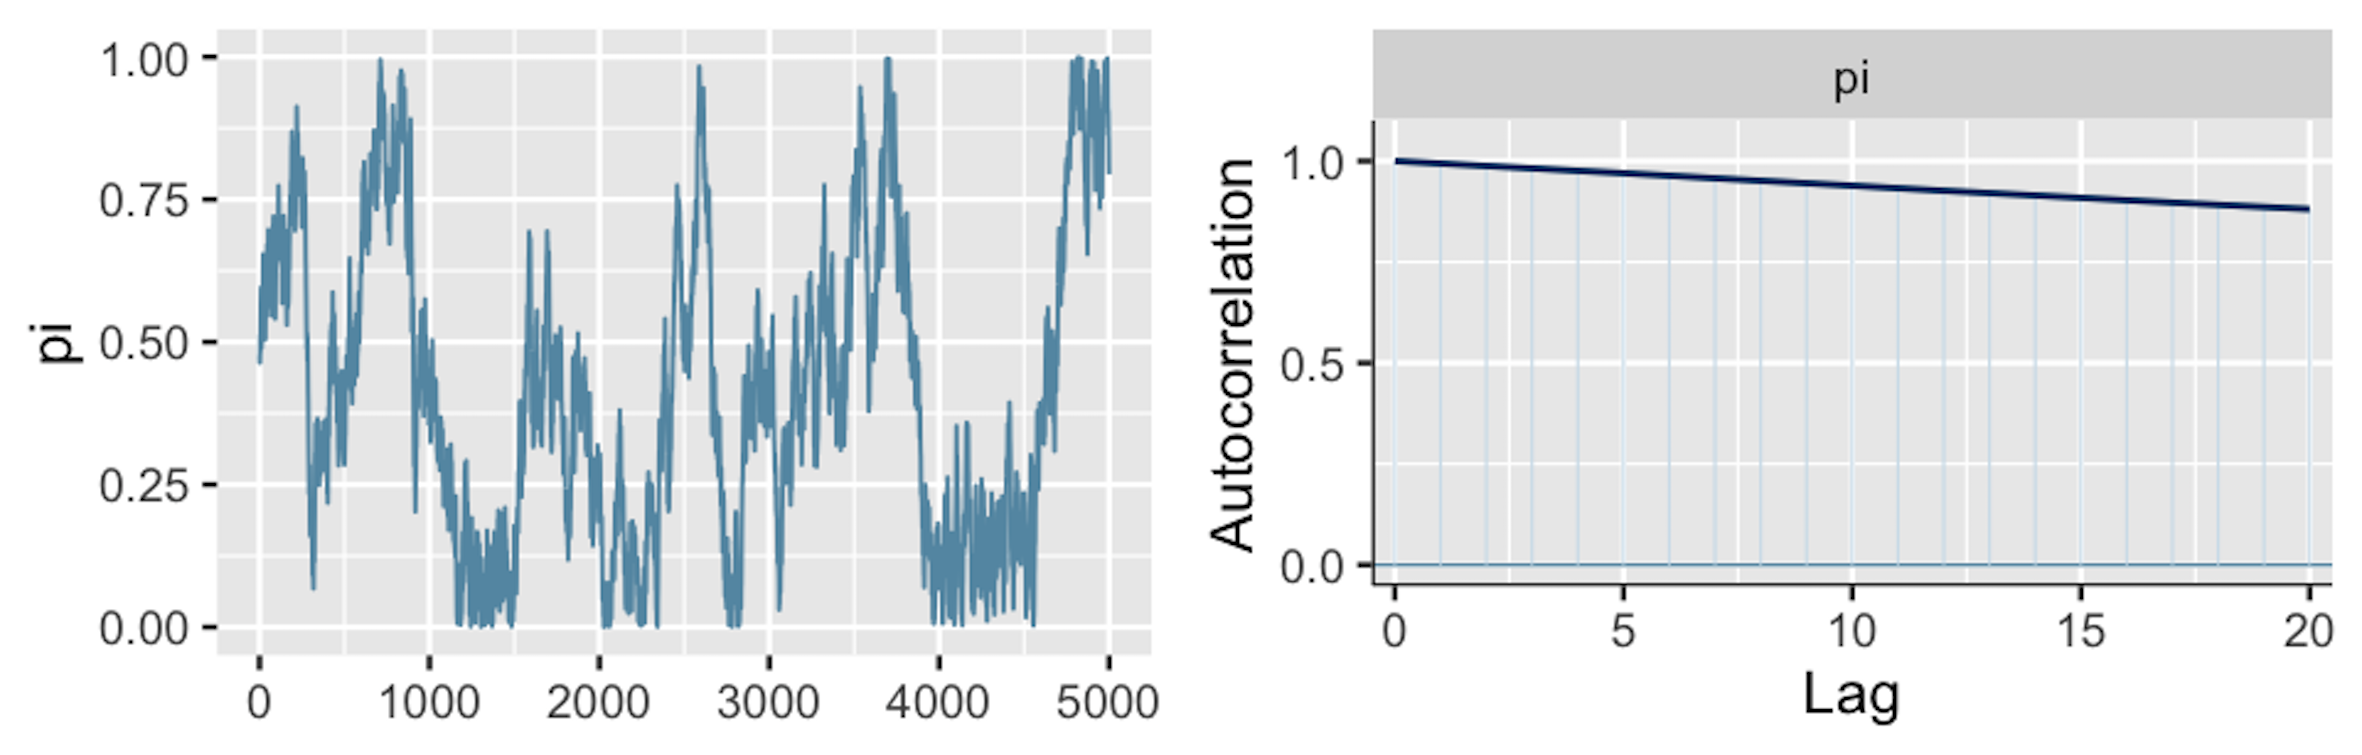
\includegraphics[width=32.81in]{images/ch6-acf-2-1} 

}

\caption{Trace plot (a sinistra) e correlogramma (a destra) di una catena di Markow in cui il mixing è lento -- figura riprodotta da @Johnson2022bayesrules.}\label{fig:bad-autocorrelation}
\end{figure}

Questa osservazione è confermata nell'correlogramma (a destra). La lenta diminuzione della curva di autocorrelazione indica che la dipendenza tra i valori della catena non svanisce rapidamente. Con un lag di 20 la correlazione è addirittura pari a 0.9. Poiché i valori della catena sono fortemente associati tra loro, il ``mixing'' è lento: la simulazione richiede un numero molto grande di iterazioni per esplorare adeguatamente l'intera gamma di valori della distribuzione a posteriori.\footnote{Una (famiglia di) catene di Markov è \emph{rapidly mixing} se mostra un comportamento simile a quello di un campione indipendente: i valori delle catene si addensano nell'intervallo dei valori più plausibili della distribuzione a posteriori; l'autocorrelazione tra i valori della catena diminuisce rapidamente; il rapporto campionario effettivo è ragionevolmente grande. Le catene che non sono \emph{rapidly mixing} non godono delle caratteristiche di un campione indipendente: le catene non si addensano nell'intervallo dei valori più plausibili della distribuzione a posteriori; l'autocorrelazione tra i valori della catena diminuisce molto lentamente; il rapporto campionario effettivo è piccolo.}

In presenza di catene di Markov non \emph{rapidly mixing} sono possibili due rimedi.

\begin{itemize}
\tightlist
\item
  Aumentare il numero di iterazioni. Anche una catena non \emph{rapidly mixing} può produrre eventualmente una buona approssimazione della distribuzione a posteriori se il numero di iterazioni è sufficientemente grande.
\item
  \emph{Thinning}. Per esempio, se la catena di Markov è costituita da 16000 valori di \(\theta\), potremmo decidere di conservare solo ogni secondo valore e ignorare gli altri valori: \(\{\theta^{(2)}, \theta^{(4)}, \theta^{(6)}, \dots, \theta^{(16000)}\}\). Oppure, potremmo decidere di conservare ogni decimo valore: \(\{\theta^{(10)}, \theta^{(20)}, \theta^{(30)}, \dots, \theta^{(16000)}\}\). Scartando i campioni intermedi, è possibile rimuovere le forti correlazioni che sono presenti nel caso di lag più piccoli.
\end{itemize}

Vediamo ora come sia possibile estrarre i valodi di una catena dall'oggetto \texttt{stanfit1}.

\begin{Shaded}
\begin{Highlighting}[]
\CommentTok{\# valori delle 4 catene}
\NormalTok{S }\OtherTok{\textless{}{-}}\NormalTok{ ggmcmc}\SpecialCharTok{::}\FunctionTok{ggs}\NormalTok{(stanfit1)}
\FunctionTok{head}\NormalTok{(S)}
\CommentTok{\#\textgreater{} \# A tibble: 6 x 4}
\CommentTok{\#\textgreater{}   Iteration Chain Parameter value}
\CommentTok{\#\textgreater{}       \textless{}dbl\textgreater{} \textless{}int\textgreater{} \textless{}fct\textgreater{}     \textless{}dbl\textgreater{}}
\CommentTok{\#\textgreater{} 1         1     1 theta     0.833}
\CommentTok{\#\textgreater{} 2         2     1 theta     0.822}
\CommentTok{\#\textgreater{} 3         3     1 theta     0.633}
\CommentTok{\#\textgreater{} 4         4     1 theta     0.798}
\CommentTok{\#\textgreater{} 5         5     1 theta     0.855}
\CommentTok{\#\textgreater{} 6         6     1 theta     0.909}
\end{Highlighting}
\end{Shaded}

\noindent
La prima catena può essere isolata nel modo seguente:

\begin{Shaded}
\begin{Highlighting}[]
\NormalTok{S1 }\OtherTok{\textless{}{-}}\NormalTok{ S }\SpecialCharTok{\%\textgreater{}\%}
\NormalTok{  dplyr}\SpecialCharTok{::}\FunctionTok{filter}\NormalTok{(}
\NormalTok{    Chain }\SpecialCharTok{==} \DecValTok{1}\NormalTok{,}
\NormalTok{    Parameter }\SpecialCharTok{==} \StringTok{"theta"}
\NormalTok{  )}
\end{Highlighting}
\end{Shaded}

\noindent
Una serie temporale della catena si ottiene con la funzione \texttt{ggmcmc::ggs\_running}:

\begin{Shaded}
\begin{Highlighting}[]
\NormalTok{ggmcmc}\SpecialCharTok{::}\FunctionTok{ggs\_running}\NormalTok{(S1)}
\end{Highlighting}
\end{Shaded}

\begin{center}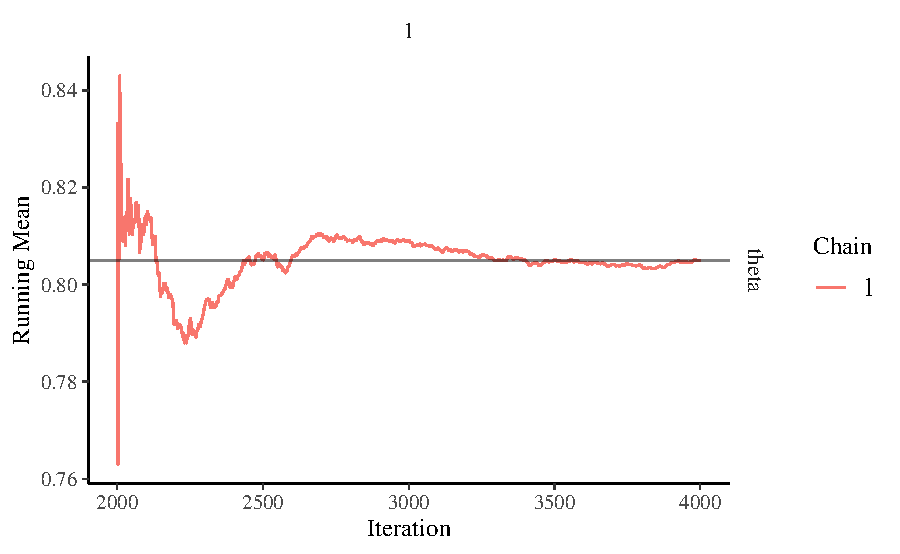
\includegraphics{041_diagnostica_MCMC_files/figure-latex/unnamed-chunk-11-1} \end{center}

\noindent
Il grafico precedente mostra che, per il modello bayesiano che stiamo discutendo, una condizione di equilibrio della catena di Markov richiederebbe un numero maggiore di iterazioni di quelle che sono state effettivamente simulate.

L'autocorrelazione di ordine 1 si ottiene nel modo seguente (si veda il Paragrafo \ref{approx-post-autocor}):

\begin{Shaded}
\begin{Highlighting}[]
\FunctionTok{cor}\NormalTok{(S1}\SpecialCharTok{$}\NormalTok{value[}\SpecialCharTok{{-}}\FunctionTok{length}\NormalTok{(S1}\SpecialCharTok{$}\NormalTok{value)], S1}\SpecialCharTok{$}\NormalTok{value[}\SpecialCharTok{{-}}\DecValTok{1}\NormalTok{])}
\CommentTok{\#\textgreater{} [1] 0.471083}
\end{Highlighting}
\end{Shaded}

\noindent
Questo valore corrisponde a ciò che è riportato nel correlogramma mostrato sopra.

\hypertarget{statistica-hatr}{%
\section{\texorpdfstring{Statistica \(\hat{R}\)}{Statistica \textbackslash hat\{R\}}}\label{statistica-hatr}}

In precedenza abbiamo detto che non solo è necessario che ogni singola catena sia stazionaria, è anche necessario che le diverse catene siano coerenti tra loro. La statistica \(\hat{R}\) affronta questo problema calcolando il rapporto tra la varianza tra le catene markoviane e la varianza entro le catene. In una situazione ottimale \(\hat{R} = 1\); se \(\hat{R}\) è lontano da 1 questo vuol dire che non è ancora stata raggiunta la convergenza.

È possibile calcolare \(\hat{R}\) mediante la chiamata alla funzione \texttt{bayesplot::rhat()}. Per il modello Beta-Binomiale applicato ai dati di \textcite{Gautret_2020} abbiamo:

\begin{Shaded}
\begin{Highlighting}[]
\NormalTok{bayesplot}\SpecialCharTok{::}\FunctionTok{rhat}\NormalTok{(stanfit1, }\AttributeTok{pars =} \StringTok{"theta"}\NormalTok{)}
\CommentTok{\#\textgreater{} [1] 1.000499}
\end{Highlighting}
\end{Shaded}

\noindent
il che indica che il valore \(\hat{R}\) ottenuto è molto simile al valore ottimale.

In maniera euristica, si può affermare che se \(\hat{R}\) supera la soglia di 1.05 questo viene interpretato come evidenza che le diverse catene parallele non producono approssimazioni coerenti della distribuzione a posteriori, quindi la simulazione è instabile.

Una rappresentazione grafica dei valori \(\hat{R}\) per tutti i parametri del modello si ottiene con la seguente chiamata:

\begin{Shaded}
\begin{Highlighting}[]
\NormalTok{ggmcmc}\SpecialCharTok{::}\FunctionTok{ggs\_Rhat}\NormalTok{(S) }\SpecialCharTok{+} \FunctionTok{xlab}\NormalTok{(}\StringTok{"R\_hat"}\NormalTok{) }\SpecialCharTok{+} \FunctionTok{xlim}\NormalTok{(}\FloatTok{0.95}\NormalTok{, }\FloatTok{1.05}\NormalTok{)}
\end{Highlighting}
\end{Shaded}

\begin{center}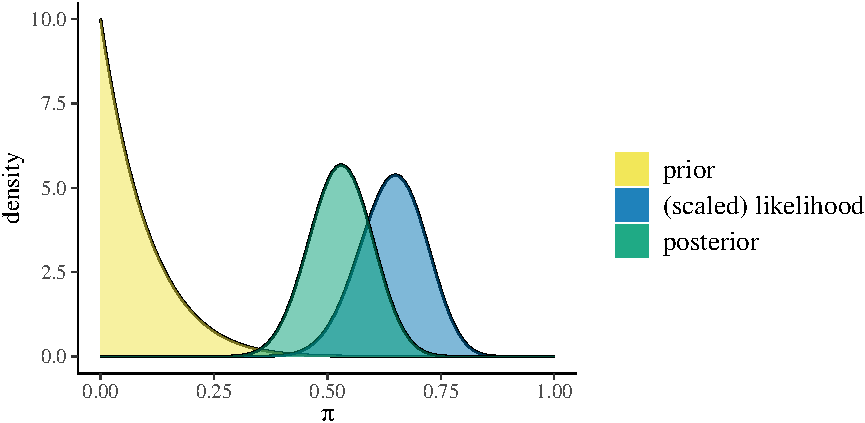
\includegraphics{041_diagnostica_MCMC_files/figure-latex/unnamed-chunk-14-1} \end{center}

\hypertarget{diagnostica-di-convergenza-di-geweke}{%
\section{Diagnostica di convergenza di Geweke}\label{diagnostica-di-convergenza-di-geweke}}

La statistica diagnostica di convergenza di Geweke è basata su un test per l'uguaglianza delle medie della prima e dell'ultima parte di una catena di Markov (di default il primo 10\% e l'ultimo 50\% della catena). Se i due campioni sono estratti dalla distribuzione stazionaria della catena, le due medie sono statisticamente uguali e la statistica di Geweke ha una distribuzione asintotica Normale standardizzata.

Utilizzando l'oggetto \texttt{stanfit1}, possiamo recuperare la statistica di Geweke nel modo seguente:

\begin{Shaded}
\begin{Highlighting}[]
\NormalTok{fit\_mcmc }\OtherTok{\textless{}{-}} \FunctionTok{As.mcmc.list}\NormalTok{(}
\NormalTok{  stanfit1,}
  \AttributeTok{pars =} \FunctionTok{c}\NormalTok{(}\StringTok{"theta"}\NormalTok{)}
\NormalTok{)}
\NormalTok{coda}\SpecialCharTok{::}\FunctionTok{geweke.diag}\NormalTok{(fit\_mcmc, }\AttributeTok{frac1 =}\NormalTok{ .}\DecValTok{1}\NormalTok{, }\AttributeTok{frac2 =}\NormalTok{ .}\DecValTok{5}\NormalTok{)}
\CommentTok{\#\textgreater{} [[1]]}
\CommentTok{\#\textgreater{} }
\CommentTok{\#\textgreater{} Fraction in 1st window = 0.1}
\CommentTok{\#\textgreater{} Fraction in 2nd window = 0.5 }
\CommentTok{\#\textgreater{} }
\CommentTok{\#\textgreater{}   theta }
\CommentTok{\#\textgreater{} {-}0.8403 }
\CommentTok{\#\textgreater{} }
\CommentTok{\#\textgreater{} }
\CommentTok{\#\textgreater{} [[2]]}
\CommentTok{\#\textgreater{} }
\CommentTok{\#\textgreater{} Fraction in 1st window = 0.1}
\CommentTok{\#\textgreater{} Fraction in 2nd window = 0.5 }
\CommentTok{\#\textgreater{} }
\CommentTok{\#\textgreater{}  theta }
\CommentTok{\#\textgreater{} 0.0759 }
\CommentTok{\#\textgreater{} }
\CommentTok{\#\textgreater{} }
\CommentTok{\#\textgreater{} [[3]]}
\CommentTok{\#\textgreater{} }
\CommentTok{\#\textgreater{} Fraction in 1st window = 0.1}
\CommentTok{\#\textgreater{} Fraction in 2nd window = 0.5 }
\CommentTok{\#\textgreater{} }
\CommentTok{\#\textgreater{}   theta }
\CommentTok{\#\textgreater{} {-}0.7616 }
\CommentTok{\#\textgreater{} }
\CommentTok{\#\textgreater{} }
\CommentTok{\#\textgreater{} [[4]]}
\CommentTok{\#\textgreater{} }
\CommentTok{\#\textgreater{} Fraction in 1st window = 0.1}
\CommentTok{\#\textgreater{} Fraction in 2nd window = 0.5 }
\CommentTok{\#\textgreater{} }
\CommentTok{\#\textgreater{} theta }
\CommentTok{\#\textgreater{} 1.878}
\end{Highlighting}
\end{Shaded}

\noindent
Per interpretare questi valori ricordiamo che la statistica di Geweke è uguale a zero quando le medie delle due porzioni della catena di Markov sono uguali. Valori maggiori di \(\mid 2 \mid\) suggeriscono che la catena non ha ancora raggiunto una distribuzione stazionaria.

\hypertarget{chapter-sintesi-distr-post}{%
\chapter{Sintesi a posteriori}\label{chapter-sintesi-distr-post}}

La distribuzione a posteriori è un modo per descrivere il nostro grado
di incertezza rispetto al parametro incognito (o rispetto ai parametri
incogniti) oggetto dell'inferenza. La distribuzione a posteriori
contiene tutte le informazioni disponibili sui possibili valori del
parametro. Se il parametro esaminato è monodimensionale (o
bidimensionale) è possibile fornire un grafico di tutta la distribuzione a posteriori \(p(\theta \mid y)\). Tuttavia, spesso vogliamo anche giungere ad una sintesi numerica della distribuzione a posteriori, soprattutto se il vettore dei parametri ha più di due dimensioni. A a questo proposito è possibile utilizzare le consuete statistiche descrittive, come media, mediana, moda, varianza, deviazione standard e i quantili. In alcuni casi, queste statistiche descrittive sono più facili da presentare e interpretare rispetto alla rappresentazione grafica della distribuzione a posteriori.

La stima puntuale della tendenza centrale della distribuzione a posteriori fornisce informazioni su quello che può essere considerato come il ``valore più plausibile'' del parametro. L'intervallo di credibilità fornisce invece un'indicazione dell'ampiezza dell'intervallo che contiene una determinata quota della massa della distribuzione a posteriori del parametro.

\hypertarget{stima-puntuale}{%
\section{Stima puntuale}\label{stima-puntuale}}

Per sintetizzare la distribuzione a posteriori in modo da giungere ad
una stima puntuale di \(\theta\) si è soliti scegliere tra moda, mediana o media a seconda del tipo di distribuzione con cui si ha a che fare e
della sua forma. Ogni stima puntuale ha una sua interpretazione.

\begin{itemize}
\tightlist
\item
  La media è il valore atteso a posteriori del parametro.
\item
  La moda può essere interpretata come il singolo valore più credibile (``più plausibile'') del parametro, alla luce dei dati, ovvero il valore per il parametro \(\theta\) che massimizza la distribuzione a posteriori. Per questa ragione la moda viene detta \emph{massimo a posteriori}, MAP. Il limite della moda quale statistica riassuntiva della distribuzione a posteriori è che, talvolta, tale distribuzione è multimodale e il MAP non è necessariamente il valore ``più credibile''.
\item
  La mediana è il valore del parametro tale per cui, su entrambi i lati di essa, giace il 50\% della massa di probabilità a posteriori.
\end{itemize}

La misura di variabilità del parametro è la \emph{varianza a posteriori}
la quale, nel caso di una distribuzione a posteriori ottenuta per via
numerica, si calcola con la formula della varianza che conosciamo
rispetto alla tendenza centrale data dalla media a posteriori. La radice quadrata della varianza a posteriori è la \emph{deviazione standard a posteriori} che descrive l'incertezza a posteriori circa il parametro di interesse nella stessa unità di misura dei dati.

Le procedure bayesiane basate sui metodi MCMC utilizzano un numero finito di campioni dalla distribuzione stazionaria, e una tale caratteristica della simulazione introduce un ulteriore livello di incertezza nella stima del parametro. L'\emph{errore standard della stima} (in inglese \emph{Monte Carlo standard error}, MCSE) misura l'accuratezza della simulazione. La deviazione standard a posteriori e l'errore standard della stima sono due concetti completamente diversi. La deviazione standard a posteriori descrive l'incertezza circa il parametro (l'ampiezza della distribuzione a posteriori) ed è una funzione della dimensione del campione; il MCSE descrive invece l'incertezza nella stima del parametro dovuta alla simulazione MCMC ed è una funzione del numero di iterazioni nella simulazione.

\hypertarget{intervallo-di-credibilituxe0}{%
\section{Intervallo di credibilità}\label{intervallo-di-credibilituxe0}}

Molto spesso la stima puntuale è accompagnata da una stima intervallare. Nella statistica bayesiana, se il parametro \(\theta \in \Theta\) è monodimensionale, si dice \emph{intervallo di credibilità} un intervallo di valori \(I_{\alpha}\) che contiene la proporzione \(1 - \alpha\) della massa di probabilità della funzione a posteriori:

\begin{equation}
p(\Theta \in I_{\alpha} \mid y) = 1 - \alpha.
\label{eq:credibint}
\end{equation}

L'intervallo di credibilità ha lo scopo di esprimere il nostro grado di incertezza riguardo la stima del parametro. Se il parametro \(\theta\) è multidimensionale, si parla invece di ``regione di credibilità''.

La condizione \eqref{eq:credibint} non determina un unico intervallo di
credibilità al \((1 - \alpha) \cdot 100\%\). In realtà esiste un numero
infinito di tali intervalli. Ciò significa che dobbiamo definire alcune
condizioni aggiuntive per la scelta dell'intervallo di credibilità.
Esaminiamo due delle condizioni aggiuntive più comuni.

\hypertarget{intervallo-di-credibilituxe0-a-code-uguali}{%
\subsection{Intervallo di credibilità a code uguali}\label{intervallo-di-credibilituxe0-a-code-uguali}}

Un intervallo di credibilità \emph{a code uguali} a livello \(\alpha\) è un
intervallo \[I_{\alpha} = [q_{\alpha/2}, 1 - q_{\alpha/2}],\] dove \(q_z\) è un quantile \(z\) della distribuzione a posteriori. Per esempio,
l'intervallo di credibilità a code uguali al 95\% è un intervallo

\[
I_{0.05} = [q_{0.025}, q_{0.975}]
\]

che lascia il 2.5\% della massa di densità a posteriori in ciascuna coda.

\hypertarget{intervallo-di-credibilituxe0-a-densituxe0-a-posteriori-piuxf9-alta}{%
\subsection{Intervallo di credibilità a densità a posteriori più alta}\label{intervallo-di-credibilituxe0-a-densituxe0-a-posteriori-piuxf9-alta}}

Nell'intervallo di credibilità a code uguali alcuni valori del parametro che sono inclusi nell'intervallo possono avere una credibilità a posteriori più bassa rispetto a quelli esterni all'intervallo. L'intrevallo di credibilità \emph{a densità a posteriori più alta} (in inglese \emph{High Posterior Density Interval}, HPD) è invece costruito in modo tale da assicurare di includere nell'intervallo tutti i valori \(\theta\) che sono a posteriori maggiormente credibili. Graficamente questo intervallo può essere ricavato tracciando una linea orizzontale sulla rappresentazione della distribuzione a posteriori e regolando l'altezza della linea in modo tale che l'area sottesa alla curva sia pari a \(1 - \alpha\). Questo tipo di intervallo è il più stretto possibile, tra tutti i possibili intervalli di credibilità allo stesso livello di fiducia. Se la distribuzione a posteriori è simmetrica unimodale, l'intervallo di credibilità a densità a posteriori più alta corrisponde all'intervallo di credibilità a code uguali.

\hypertarget{interpretazione}{%
\subsection{Interpretazione}\label{interpretazione}}

L'interpretazione dell'intervallo di credibilità è molto intuitiva:
l'intervallo di credibilità è un intervallo di valori all'interno del
quale cade il valore del parametro incognito con un particolare livello
di probabilità soggettiva. Possiamo dire che, dopo aver visto i dati
crediamo, con un determinato livello di probabilità soggettiva, che il
valore del parametro (ad esempio, la dimensione dell'effetto di un
trattamento) abbia un valore compreso all'interno dell'intervallo che è
stato calcolato, laddove per probabilità soggettiva intendiamo ``il grado di fiducia che lo sperimentatore ripone nel verificarsi di un evento''. Gli intervalli di credibilità si calcolano con un software.

\hypertarget{un-esempio-concreto}{%
\section{Un esempio concreto}\label{un-esempio-concreto}}

Per fare un esempio pratico, consideriamo nuovamente i valori del BDI-II dei 30 soggetti clinici di \textcite{zetschefuture2019}:

\begin{Shaded}
\begin{Highlighting}[]
\FunctionTok{suppressPackageStartupMessages}\NormalTok{(}\FunctionTok{library}\NormalTok{(}\StringTok{"bayesrules"}\NormalTok{))}

\NormalTok{df }\OtherTok{\textless{}{-}} \FunctionTok{data.frame}\NormalTok{(}
  \AttributeTok{y =} \FunctionTok{c}\NormalTok{(}
    \DecValTok{26}\NormalTok{, }\DecValTok{35}\NormalTok{, }\DecValTok{30}\NormalTok{, }\DecValTok{25}\NormalTok{, }\DecValTok{44}\NormalTok{, }\DecValTok{30}\NormalTok{, }\DecValTok{33}\NormalTok{, }\DecValTok{43}\NormalTok{, }\DecValTok{22}\NormalTok{, }\DecValTok{43}\NormalTok{,}
    \DecValTok{24}\NormalTok{, }\DecValTok{19}\NormalTok{, }\DecValTok{39}\NormalTok{, }\DecValTok{31}\NormalTok{, }\DecValTok{25}\NormalTok{, }\DecValTok{28}\NormalTok{, }\DecValTok{35}\NormalTok{, }\DecValTok{30}\NormalTok{, }\DecValTok{26}\NormalTok{, }\DecValTok{31}\NormalTok{,}
    \DecValTok{41}\NormalTok{, }\DecValTok{36}\NormalTok{, }\DecValTok{26}\NormalTok{, }\DecValTok{35}\NormalTok{, }\DecValTok{33}\NormalTok{, }\DecValTok{28}\NormalTok{, }\DecValTok{27}\NormalTok{, }\DecValTok{34}\NormalTok{, }\DecValTok{27}\NormalTok{, }\DecValTok{22}
\NormalTok{  )}
\NormalTok{)}
\end{Highlighting}
\end{Shaded}

Un valore BDI-II \(\geq 30\) indica la presenza di un livello ``grave'' di depressione. Nel campione clinico di \textcite{zetschefuture2019},

\begin{Shaded}
\begin{Highlighting}[]
\FunctionTok{sum}\NormalTok{(df}\SpecialCharTok{$}\NormalTok{y }\SpecialCharTok{\textgreater{}} \DecValTok{29}\NormalTok{)}
\CommentTok{\#\textgreater{} [1] 17}
\end{Highlighting}
\end{Shaded}

\noindent
17 pazienti su 30 manifestano un livello grave di depressione.

Supponiamo di volere stimare la distribuzione a posteriori della probabilità \(\theta\) di depressione ``grave'' nei pazienti clinici, così come viene misurata dal test BDI-II, imponendo su \(\theta\) una distribuzione a priori \(\mbox{Beta}(8, 2)\).

Sappiamo che il modello Beta-Binomiale può essere espresso nella forma seguente:

\begin{align}
Y | \theta & \sim \mbox{Bin}(30, \theta) \notag\\
\theta & \sim \mbox{Beta}(8, 2) \notag
\end{align}

\noindent
con una corrispondente distribuzione a posteriori \(\mbox{Beta}(25, 15)\):

\begin{equation}
f(\theta | y = 17) = \frac{\Gamma(25 + 15)}{\Gamma(25)\Gamma(15)}\theta^{25-1} (1-\theta)^{15-1} \;\; \text{ for } \theta \in [0,1] \; .
\label{eq:post-beta-25-15}
\end{equation}

\begin{Shaded}
\begin{Highlighting}[]
\FunctionTok{plot\_beta\_binomial}\NormalTok{(}\AttributeTok{alpha =} \DecValTok{8}\NormalTok{, }\AttributeTok{beta =} \DecValTok{2}\NormalTok{, }\AttributeTok{y =} \DecValTok{17}\NormalTok{, }\AttributeTok{n =} \DecValTok{30}\NormalTok{)}
\end{Highlighting}
\end{Shaded}

\begin{center}\includegraphics{045_summarize_posterior_files/figure-latex/unnamed-chunk-4-1} \end{center}

\hypertarget{stime-puntuali-della-distribuzione-a-posteriori}{%
\subsection{Stime puntuali della distribuzione a posteriori}\label{stime-puntuali-della-distribuzione-a-posteriori}}

Una volta trovata l'intera distribuzione a posteriori, quale valore di
sintesi è necessario riportare? Questa sembra una domanda innocente, ma
in realtà è una domanda a cui è difficile rispondere. La stima bayesiana dei parametri è fornita dall'intera distribuzione a posteriori, che non è un singolo numero, ma una funzione che mappa ciascun valore del parametro ad un valore di plausibilità. Quindi non è necessario scegliere una stima puntuale. In linea di principio, una stima puntuale non è quasi mai necessaria ed è spesso dannosa in quanto comporta una perdita di informazioni.

Tuttavia talvolta una tale sintesi è richiesta. Diverse risposte sono allora possibili. La media della distribuzione a posteriori per \(\theta\) è

\[
\E(\pi \mid y = 17) = \frac{\alpha}{\alpha + \beta} = \frac{25}{25+15} = 0.625.
\]

Una stima del massimo della probabilità a posteriori, o brevemente massimo a posteriori, MAP (da \emph{maximum a posteriori probability}), è la moda della distribuzione a posteriori. Nel caso presente, una stima del MAP può essere ottenuta nel modo seguente:

\[
\Mo(\pi \mid y = 17) = \frac{\alpha-1}{\alpha + \beta-2} = \frac{25-1}{25+15-2} = 0.6316.
\]

Gli stessi risultati si ottiengono usando la chiamata a \texttt{bayesrules::summarize\_beta\_binomial()}:

\begin{Shaded}
\begin{Highlighting}[]
\FunctionTok{summarize\_beta\_binomial}\NormalTok{(}\AttributeTok{alpha =} \DecValTok{8}\NormalTok{, }\AttributeTok{beta =} \DecValTok{2}\NormalTok{, }\AttributeTok{y =} \DecValTok{17}\NormalTok{, }\AttributeTok{n =} \DecValTok{30}\NormalTok{)}
\CommentTok{\#\textgreater{}       model alpha beta  mean      mode         var}
\CommentTok{\#\textgreater{} 1     prior     8    2 0.800 0.8750000 0.014545455}
\CommentTok{\#\textgreater{} 2 posterior    25   15 0.625 0.6315789 0.005716463}
\CommentTok{\#\textgreater{}          sd}
\CommentTok{\#\textgreater{} 1 0.1206045}
\CommentTok{\#\textgreater{} 2 0.0756073}
\end{Highlighting}
\end{Shaded}

La mediana si ottiene con

\begin{Shaded}
\begin{Highlighting}[]
\FunctionTok{qbeta}\NormalTok{(.}\DecValTok{5}\NormalTok{, }\AttributeTok{shape1 =} \DecValTok{25}\NormalTok{, }\AttributeTok{shape2 =} \DecValTok{15}\NormalTok{)}
\CommentTok{\#\textgreater{} [1] 0.6271031}
\end{Highlighting}
\end{Shaded}

\hypertarget{intervallo-di-credibilituxe0-1}{%
\subsection{Intervallo di credibilità}\label{intervallo-di-credibilituxe0-1}}

È più comune sintetizzare la distribuzione a posteriori mediante l'intervallo di credibilità. Per esempio, l'intervallo di credibilità a code uguali al 95\%

\begin{Shaded}
\begin{Highlighting}[]
\FunctionTok{plot\_beta\_ci}\NormalTok{(}\AttributeTok{alpha =} \DecValTok{25}\NormalTok{, }\AttributeTok{beta =} \DecValTok{15}\NormalTok{, }\AttributeTok{ci\_level =} \FloatTok{0.95}\NormalTok{)}
\end{Highlighting}
\end{Shaded}

\begin{center}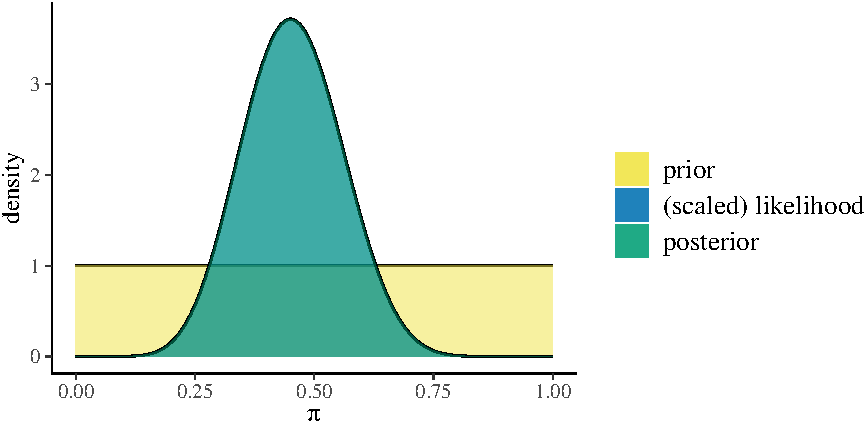
\includegraphics{045_summarize_posterior_files/figure-latex/unnamed-chunk-7-1} \end{center}

\noindent
è dato dalla chiamata

\begin{Shaded}
\begin{Highlighting}[]
\FunctionTok{qbeta}\NormalTok{(}\FunctionTok{c}\NormalTok{(}\FloatTok{0.025}\NormalTok{, }\FloatTok{0.975}\NormalTok{), }\DecValTok{25}\NormalTok{, }\DecValTok{15}\NormalTok{)}
\CommentTok{\#\textgreater{} [1] 0.4717951 0.7663607}
\end{Highlighting}
\end{Shaded}

\noindent
Il calcolo precedente evidenzia l'interpretazione intuitiva dell'intervallo di credibilità. Tale intervallo, infatti, può essere interpretato come la probabilità che \(\theta\) assuma valori compresi tra 0.472 e 0.766:

\[
P(\theta \in (0.472, 0.766) | Y = 17) = \int_{0.472}^{0.766} f(\theta \mid y=17) d\theta = 0.95,
\]

\noindent
ovvero

\begin{Shaded}
\begin{Highlighting}[]
\NormalTok{postFun }\OtherTok{\textless{}{-}} \ControlFlowTok{function}\NormalTok{(theta) \{}
  \FunctionTok{gamma}\NormalTok{(}\DecValTok{25} \SpecialCharTok{+} \DecValTok{15}\NormalTok{) }\SpecialCharTok{/}\NormalTok{ (}\FunctionTok{gamma}\NormalTok{(}\DecValTok{25}\NormalTok{) }\SpecialCharTok{*} \FunctionTok{gamma}\NormalTok{(}\DecValTok{15}\NormalTok{)) }\SpecialCharTok{*}\NormalTok{ theta}\SpecialCharTok{\^{}}\DecValTok{24} \SpecialCharTok{*}\NormalTok{ (}\DecValTok{1} \SpecialCharTok{{-}}\NormalTok{ theta)}\SpecialCharTok{\^{}}\DecValTok{14}
\NormalTok{\}}
\FunctionTok{integrate}\NormalTok{(}
\NormalTok{  postFun,}
  \AttributeTok{lower =} \FloatTok{0.4717951}\NormalTok{,}
  \AttributeTok{upper =} \FloatTok{0.7663607}
\NormalTok{)}\SpecialCharTok{$}\NormalTok{value}
\CommentTok{\#\textgreater{} [1] 0.95}
\end{Highlighting}
\end{Shaded}

Possiamo costruire diversi intervalli di credibilità a code equivalenti. Ad esempio, l'intervallo di credibilità compreso tra il 25-esimo e il 75-esimo percentile è

\begin{Shaded}
\begin{Highlighting}[]
\FunctionTok{qbeta}\NormalTok{(}\FunctionTok{c}\NormalTok{(}\FloatTok{0.25}\NormalTok{, }\FloatTok{0.75}\NormalTok{), }\DecValTok{25}\NormalTok{, }\DecValTok{15}\NormalTok{)}
\CommentTok{\#\textgreater{} [1] 0.5743878 0.6778673}
\end{Highlighting}
\end{Shaded}

\noindent
ovvero, abbiamo una certezza a posteriori del 50\% che la probabilità di depressione grave tra i pazienti clinici sia un valore compreso tra 0.57 e 0.68.

Non esiste un livello credibile ``corretto''. I ricercatori, utilizzano vari livelli, ad esempio 50\%, 80\% o 95\%, a seconda del contesto dell'analisi. Ciascuno di questi intervalli fornisce un'immagine diversa della nostra comprensione della distribuzione a posteriori del parametro di interesse.

Non è inoltre necessario riportare l'intervallo di credibilità a code uguali. Se la distribuzione a posteriori è fortemente asimmetrica è più sensato riportare l'intervallo di credibilità a densità a posteriori più alta.
L'intervallo HPD risulta più semplice da determinare quando la distribuzione a posteriori viene approssimata con il metodo MCMC.

\hypertarget{probabilituxe0-della-distribuzione-a-posteriori}{%
\subsection{Probabilità della distribuzione a posteriori}\label{probabilituxe0-della-distribuzione-a-posteriori}}

Il test di ipotesi è un compito comune dell'analisi della distribuzione a posteriori. Supponiamo che si voglia conoscere la probabilità a posteriori che \(\theta\) sia superiore a 0.5. Per sapere quanto credibile sia l'evento \(\theta > 0.5\) possiamo calcolare il seguente integrale:

\[
P(\theta > 0.5 \; \mid \; y = 17) = \int_{0.5}^{1}f(\theta \mid y=17)d\theta \;,
\]

\noindent
dove \(f(\cdot)\) è la distribuzione \(\mbox{\Beta}(25, 15)\):

\begin{Shaded}
\begin{Highlighting}[]
\FunctionTok{pbeta}\NormalTok{(}\FloatTok{0.5}\NormalTok{, }\AttributeTok{shape1 =} \DecValTok{25}\NormalTok{, }\AttributeTok{shape2 =} \DecValTok{15}\NormalTok{, }\AttributeTok{lower.tail =} \ConstantTok{FALSE}\NormalTok{)}
\CommentTok{\#\textgreater{} [1] 0.9459355}
\end{Highlighting}
\end{Shaded}

\noindent
il che è equivalente a:

\begin{Shaded}
\begin{Highlighting}[]
\NormalTok{postFun }\OtherTok{\textless{}{-}} \ControlFlowTok{function}\NormalTok{(theta) \{}
  \FunctionTok{gamma}\NormalTok{(}\DecValTok{25} \SpecialCharTok{+} \DecValTok{15}\NormalTok{) }\SpecialCharTok{/}\NormalTok{ (}\FunctionTok{gamma}\NormalTok{(}\DecValTok{25}\NormalTok{) }\SpecialCharTok{*} \FunctionTok{gamma}\NormalTok{(}\DecValTok{15}\NormalTok{)) }\SpecialCharTok{*}\NormalTok{ theta}\SpecialCharTok{\^{}}\DecValTok{24} \SpecialCharTok{*}\NormalTok{ (}\DecValTok{1} \SpecialCharTok{{-}}\NormalTok{ theta)}\SpecialCharTok{\^{}}\DecValTok{14}
\NormalTok{\}}
\FunctionTok{integrate}\NormalTok{(}
\NormalTok{  postFun,}
  \AttributeTok{lower =} \FloatTok{0.5}\NormalTok{,}
  \AttributeTok{upper =} \DecValTok{1}
\NormalTok{)}\SpecialCharTok{$}\NormalTok{value}
\CommentTok{\#\textgreater{} [1] 0.9459355}
\end{Highlighting}
\end{Shaded}

È anche possibile formulare un test di ipotesi contrastando due ipotesi contrapposte. Per esempio, \(H_1: \theta \geq 0.5\) e \(H_2: \theta < 0.5\). Ciò consente di calcolare l'\emph{odds a posteriori} di \(\theta > 0.5\):

\begin{equation}
\text{poterior odds} = \frac{H_1 \mid y = 17}{H_2 \mid y = 17}
\end{equation}

\noindent
ovvero

\begin{Shaded}
\begin{Highlighting}[]
\NormalTok{posterior\_odds }\OtherTok{\textless{}{-}}
  \FunctionTok{pbeta}\NormalTok{(}\FloatTok{0.5}\NormalTok{, }\AttributeTok{shape1 =} \DecValTok{25}\NormalTok{, }\AttributeTok{shape2 =} \DecValTok{15}\NormalTok{, }\AttributeTok{lower.tail =} \ConstantTok{FALSE}\NormalTok{) }\SpecialCharTok{/}
    \FunctionTok{pbeta}\NormalTok{(}\FloatTok{0.5}\NormalTok{, }\AttributeTok{shape1 =} \DecValTok{25}\NormalTok{, }\AttributeTok{shape2 =} \DecValTok{15}\NormalTok{, }\AttributeTok{lower.tail =} \ConstantTok{TRUE}\NormalTok{)}
\NormalTok{posterior\_odds}
\CommentTok{\#\textgreater{} [1] 17.49642}
\end{Highlighting}
\end{Shaded}

\noindent
L'odds a posteriori rappresenta l'aggiornamento delle nostre credenze dopo avere osservato \(y = 17\) in \(n = 30\). L'odds a priori di \(\theta > 0.5\) era:

\begin{Shaded}
\begin{Highlighting}[]
\NormalTok{prior\_odds }\OtherTok{\textless{}{-}}
  \FunctionTok{pbeta}\NormalTok{(}\FloatTok{0.5}\NormalTok{, }\AttributeTok{shape1 =} \DecValTok{8}\NormalTok{, }\AttributeTok{shape2 =} \DecValTok{2}\NormalTok{, }\AttributeTok{lower.tail =} \ConstantTok{FALSE}\NormalTok{) }\SpecialCharTok{/}
    \FunctionTok{pbeta}\NormalTok{(}\FloatTok{0.5}\NormalTok{, }\AttributeTok{shape1 =} \DecValTok{8}\NormalTok{, }\AttributeTok{shape2 =} \DecValTok{2}\NormalTok{, }\AttributeTok{lower.tail =} \ConstantTok{TRUE}\NormalTok{)}
\NormalTok{prior\_odds}
\CommentTok{\#\textgreater{} [1] 50.2}
\end{Highlighting}
\end{Shaded}

Il \emph{fattore di Bayes} (\emph{Bayes Factor}; BF) confronta gli odds a posteriori con gli odds a priori e quindi fornisce informazioni su quanto sia mutata la nostra comprensione relativa a \(\theta\) dopo avere osservato i nostri dati del campione:

\[
\text{BF} = \frac{\text{odds a posteriori}}{\text{odds a priori}}.
\]

\noindent
Nel caso presente abbiamo

\begin{Shaded}
\begin{Highlighting}[]
\NormalTok{BF }\OtherTok{\textless{}{-}}\NormalTok{ posterior\_odds }\SpecialCharTok{/}\NormalTok{ prior\_odds}
\NormalTok{BF}
\CommentTok{\#\textgreater{} [1] 0.3485343}
\end{Highlighting}
\end{Shaded}

Quindi, dopo avere osservato i dati, gli odds a posteriori della nostra ipotesi a proposito di \(\theta\) sono pari a solo il 34\% degli odds a priori.

Per fare un altro esempio, consideriamo invece il caso in cui le credenze a priori rivelano una credenza diametralmente opposta rispetto a \(\theta\) che nel caso considerato in precedenza, ovvero \(\mbox{Beta}(2, 8)\). In questo secondo caso, la distribuzione a posteriori diventa

\begin{Shaded}
\begin{Highlighting}[]
\FunctionTok{summarize\_beta\_binomial}\NormalTok{(}\AttributeTok{alpha =} \DecValTok{2}\NormalTok{, }\AttributeTok{beta =} \DecValTok{8}\NormalTok{, }\AttributeTok{y =} \DecValTok{17}\NormalTok{, }\AttributeTok{n =} \DecValTok{30}\NormalTok{)}
\CommentTok{\#\textgreater{}       model alpha beta  mean      mode         var}
\CommentTok{\#\textgreater{} 1     prior     2    8 0.200 0.1250000 0.014545455}
\CommentTok{\#\textgreater{} 2 posterior    19   21 0.475 0.4736842 0.006082317}
\CommentTok{\#\textgreater{}           sd}
\CommentTok{\#\textgreater{} 1 0.12060454}
\CommentTok{\#\textgreater{} 2 0.07798921}
\end{Highlighting}
\end{Shaded}

\noindent
e il BF è

\begin{Shaded}
\begin{Highlighting}[]
\NormalTok{posterior\_odds }\OtherTok{\textless{}{-}}
  \FunctionTok{pbeta}\NormalTok{(}\FloatTok{0.5}\NormalTok{, }\AttributeTok{shape1 =} \DecValTok{19}\NormalTok{, }\AttributeTok{shape2 =} \DecValTok{21}\NormalTok{, }\AttributeTok{lower.tail =} \ConstantTok{FALSE}\NormalTok{) }\SpecialCharTok{/}
    \FunctionTok{pbeta}\NormalTok{(}\FloatTok{0.5}\NormalTok{, }\AttributeTok{shape1 =} \DecValTok{19}\NormalTok{, }\AttributeTok{shape2 =} \DecValTok{21}\NormalTok{, }\AttributeTok{lower.tail =} \ConstantTok{TRUE}\NormalTok{)}

\NormalTok{prior\_odds }\OtherTok{\textless{}{-}}
  \FunctionTok{pbeta}\NormalTok{(}\FloatTok{0.5}\NormalTok{, }\AttributeTok{shape1 =} \DecValTok{2}\NormalTok{, }\AttributeTok{shape2 =} \DecValTok{8}\NormalTok{, }\AttributeTok{lower.tail =} \ConstantTok{FALSE}\NormalTok{) }\SpecialCharTok{/}
    \FunctionTok{pbeta}\NormalTok{(}\FloatTok{0.5}\NormalTok{, }\AttributeTok{shape1 =} \DecValTok{2}\NormalTok{, }\AttributeTok{shape2 =} \DecValTok{8}\NormalTok{, }\AttributeTok{lower.tail =} \ConstantTok{TRUE}\NormalTok{)}

\NormalTok{BF }\OtherTok{\textless{}{-}}\NormalTok{ posterior\_odds }\SpecialCharTok{/}\NormalTok{ prior\_odds}
\NormalTok{BF}
\CommentTok{\#\textgreater{} [1] 30.07239}
\end{Highlighting}
\end{Shaded}

\noindent
In alre parole, in questo secondo esempio gli odds a posteriori della nostra ipotesi a proposito di \(\theta\) sono aumentati di 30 volte rispetto agli odds a priori.

In generale, in un test di ipotesi che contrappone un'ipotesi sostantiva \(H_a\) ad un'ipotesi nulla \(H_0\) il BF è un rapporto di odds per l'ipotesi sostantiva:

\[
\text{Bayes Factor}
= \frac{\text{posterior odds}}{\text{prior odds}}
= \frac{P(H_a \mid Y) / P(H_0 \mid Y)}{P(H_a) / P(H_0)}
 \; .
\]

\noindent
Essendo un rapporto, il BF deve esere valutato rispetto al valore di 1. Ci sono tre possibilità:

\begin{itemize}
\tightlist
\item
  BF = 1: La credibilità di \(H_a\) non è cambiata dopo avere osservato i dati.
\item
  BF \textgreater{} 1: La credibilità di \(H_a\) è aumentata dopo avere osservato i dati. Quindi maggiore è BF, più convincente risulta l'evidenza per \(H_a\).
\item
  BF \textless{} 1: La credibilità di \(H_a\) è diminuita dopo avere osservato i dati.
\end{itemize}

Non ci sono delle soglie universalmente riconosciute per interpretare il BF. Per esempio, \textcite{lee2014bayesian} propongono il seguente schema:

\begin{longtable}[]{@{}rl@{}}
\toprule
BF & Interpretation \\
\midrule
\endhead
\textgreater{} 100 & Extreme evidence for \(H_a\) \\
30 - 100 & Very strong evidence for \(H_a\) \\
10 - 30 & Strong evidence for \(H_a\) \\
3 - 10 & Moderate evidence for \(H_a\) \\
1 - 3 & Anecdotal evidence for \(H_a\) \\
1 & No evidence \\
1/3 - 1 & Anecdotal evidence for \(H_0\) \\
1/10 - 1/3 & Moderate evidence for \(H_0\) \\
1/30 - 1/10 & Strong evidence for \(H_0\) \\
1/100 - 1/30 & Very strong evidence for \(H_0\) \\
\textless{} 1/100 & Extreme evidence for \(H_0\) \\
\bottomrule
\end{longtable}

Tuttavia, è importante notare che l'opinione maggiormente diffusa nella comunità scientifica sia quella che incoraggia a non trarre conclusioni rigide dai dati utilizzando dei criteri fissati una volta per tutte. Pertanto, non esiste una soglia univoca per il BF che consente di classificare le ipotesi dei ricercatori nelle due categorie ``vero'' o ``falso''. Invece, è più utile adottare una pratica più flessibile capace di tenere in considerazione il contesto e le potenziali implicazioni di ogni singolo test di ipotesi. Inoltre, è stato molte volte ripetuto che la distribuzione a posteriori è molto più informativa di una decisione binaria: la rappresentazione di tutta la distribuzione a posteriori fornisce una misura olistica del nostro livello di incertezza riguardo all'affermazione (il parametro, ovvero l'ipotesi) che viene valutata.

\hypertarget{considerazioni-conclusive-1}{%
\section*{Considerazioni conclusive}\label{considerazioni-conclusive-1}}
\addcontentsline{toc}{section}{Considerazioni conclusive}

Questo capitolo introduce le procedure di base per la manipolazione
della distribuzione a posteriori. Lo strumento fondamentale che è stato
utilizzato è quello fornito dai campioni di valori del parametro che vengono estratti dalla distribuzione a posteriori. Lavorare con campioni di valori del parametro estratti dalla distribuzione a posteriori trasforma un problema di calcolo integrale in un problema di riepilogo dei dati. Abbiamo visto le procedure maggiormente usate che consentono di utilizzare i campioni a
posteriori per produrre indici di sintesi della distribuzione a
posteriori: gli intervalli di credibilità e le stime puntuali.


% Bibliography
%%%%%%%%%%%%%%%%%%%%%%%%%%%%%%%%%%%%%%%%%%%%%%%%%%%%%%%%%%

\backmatter
\SmallMargins

\printbibliography
\onecolumn


% Tables (of tables, of figures)
%%%%%%%%%%%%%%%%%%%%%%%%%%%%%%%%%%%%%%%%%%%%%%%%%%%%%%%%%%


\cleardoublepage
\LargeMargins
\listoffigures


% After-body (LaTeX code inclusion)
%%%%%%%%%%%%%%%%%%%%%%%%%%%%%%%%%%%%%%%%%%%%%%%%%%%%%%%%%%




% Back cover
%%%%%%%%%%%%%%%%%%%%%%%%%%%%%%%%%%%%%%%%%%%%%%%%%%%%%%%%%%%

% Even page, small margins, no running head, no page number.
\evenpage
\SmallMargins
\thispagestyle{empty}

\begin{normalsize}

\begin{description}

\selectlanguage{italian}
\item[Abstract]
This document contains the material of the lessons of Psicometria B000286 (2021/2022) aimed at students of the first year of the Degree Course in Psychological Sciences and Techniques of the University of Florence, Italy.
\item[Keywords]
Data science, Bayesian statistics.
~\\

\end{description}

\end{normalsize}


\end{document}
